\documentclass[twoside,a4paper,openany,12pt]{book}

%%\documentclass[twoside,a4paper,12pt]{article}
%\documentclass[twoside,a4paper,openany,12pt]{report}

%% Document has convention that only first letter of chapters,
%% sections is capitalized. Do the same for automatic sections
\renewcommand\listfigurename{List of figures}
\renewcommand\listtablename{List of tables}

%% Convenient way to specify margins
\usepackage[a4paper,top=2.5cm,bottom=2.5cm,inner=2.5cm,outer=2.5cm]{geometry}

%% Relative font sizes
\usepackage{relsize}

%% Use font with 8-bit encoding
\usepackage[T1]{fontenc}

%% Nicer fonts
\usepackage{pslatex}

\usepackage{linegoal}

%% Color definitions
\usepackage{color}
\definecolor{MyLightRed}{rgb}{1,.8,.8}
\definecolor{MyCodeboxColor}{rgb}{.9,.9,.9}
\definecolor{MyLightBlue}{rgb}{.8,.8,1}
\definecolor{MyQuoteColor}{rgb}{0,.6,0}
\definecolor{MyLightMagenta}{rgb}{1,.2,1}

%% For landscape pages printed, but rotated on screen
\usepackage{pdflscape}

%% Including figures and other graphics
\usepackage{graphicx}
% \usepackage[rgb]{xcolor}
%% Rotated images etc
\usepackage{rotating}

%% Author-year citations
\usepackage[authoryear]{natbib}

%% Subfigure environment
\usepackage{subfigure}

%% Conditional sections
\usepackage{ifthen}

%% URLs
\usepackage[obeyspaces]{url}

%% SI units
\usepackage[abbreviations]{siunitx}

% Command to get a tilde which prints as an ASCII tilde in PDFs,
% needed to allow copying text and pasting into a command window or
% editor
\newcommand{\mytilde}{\texttildelow}

%% For tables align on decimal point
\usepackage{dcolumn}
\newcolumntype{d}{D{.}{.}{-1}} % centre on decimal place

%% Long tables
\usepackage{supertabular}

\usepackage{fancyhdr}

%% Alternative to verbatim. Can be used for defining new environments
\usepackage{fancyvrb}
%% A command to include Matlab files (verbatim). Surrounded with a
%% frame and smaller font size than normal. Must be defined before
%% underscore package because the custom command must be listed in
%% \UnderscoreCommands
\CustomVerbatimCommand{\IncludeMatlabFileVerb}{VerbatimInput}{frame=single,fontsize=\relsize{-1}}
\CustomVerbatimCommand{\IncludeShellFileVerb}{VerbatimInput}{frame=single,fontsize=\relsize{-1}}

%% Include Matlab file verbatim and attach it for the user to download.
\newcommand{\IncludeMatlabFile}[2]{\IncludeMatlabFileVerb{#1}%
  \attachfile[mimetype=text/plain,description=#2]{#1}}

%% Include shell file verbatim and attach it for the user to download.
\newcommand{\IncludeShellFile}[2]{\IncludeShellFileVerb{#1}%
  \attachfile[mimetype=text/plain,description=#2]{#1}}


%% Have floats on subsequent page, not miles away.
\usepackage{flafter}

\usepackage{marvosym} % for \Info
\usepackage{keystroke} % for keyboard symbols

\usepackage{abbrev}
\renewcommand{\abbrevname}{Abbreviations}
%% List of abbreviations. Include all useful ones. Those which are not
%% used are not included in the table.

\abbrev{\adc}{ADC}{analogue to digital converter}
\abbrev{\api}{API}{application programming interface}
\abbrev{\bgs}{BGS}{Bitish Geological Survey}
\abbrev{\cpu}{CPU}{central processing unit}
\abbrev{\dhcp}{DHCP}{dynamic host configuration protocol}
\abbrev{\dip}{DIP}{dual-inline package}
\abbrev{\dns}{DNS}{domain name system}
\abbrev{\dtr}{DTR}{data terminal ready}
\abbrev{\eeprom}{EEPROM}{electrically erasable programmable read-only memory}
\abbrev{\esd}{ESD}{electro-static discharge}
\abbrev{\fat}{FAT}{file allocation table}
\abbrev{\fet}{FET}{field-effect transistor}
\abbrev{\gpu}{GPU}{graphics processing unit}
\abbrev{\gui}{GUI}{graphical user interface}
\abbrev{\hmac}{HMAC}{hash-based message authentication code}
\abbrev{\http}{HTTP}{hypertext transfer protocol}
\abbrev{\https}{HTTPS}{hypertext transfer protocol secure}
\abbrev{\ic}{IC}{integrated circuit}
\abbrev{\itwoc}{I2C}{inter-integrated circuit (bus)}
\abbrev{\ir}{IR}{infra-red}
\abbrev{\ism}{ISM}{Industrical, scientific and medical (radio band)}
\abbrev{\isp}{ISP}{in-circuit serial programmer (sometimes abbreviated as ICSP)}
\abbrev{\ip}{IP}{internet protocol}
\abbrev{\jtag}{JTAG}{joint test action group}
\abbrev{\led}{LED}{light emitting diode}
\abbrev{\mdfive}{MD5}{message digest 5}
\abbrev{\nfs}{NFS}{network file system}
\abbrev{\ntp}{NTP}{network time protocol}
\abbrev{\ota}{OTA}{over the air (as in firmware updates)}
\abbrev{\pcb}{PCB}{printed circuit board}
\abbrev{\PoE}{PoE}{power over ethernet}
\abbrev{\psu}{PSU}{power supply unit}
\abbrev{\rfi}{RFI}{radio-frequency interference}
\abbrev{\rtc}{RTC}{real-time clock}
\abbrev{\samnet}{SAMNET}{Sub-Auroral Magnetometer Network}
\abbrev{\sd}{SD}{secure digital}
\abbrev{\ssh}{SSH}{secure shell}
\abbrev{\soic}{SOIC}{small outline integrated circuit}
\abbrev{\tcp}{TCP}{transmission control protocol}
\abbrev{\ttl}{TTL}{transistor-transistor logic}
%% \url is already a command, use \URL for the abbreviation
\abbrev{\URL}{URL}{uniform resource locator}
\abbrev{\usb}{USB}{universal serial bus}
\abbrev{\ut}{UT}{universal time}
\abbrev{\utc}{UTC}{coordinated universal time}
\abbrev{\udp}{UDP}{user datagram protocol}



% Load the underscore package as fixes the problem of copying and
% pasting text with underscores; previously underscores were converted
% to spaces, but they matter for code! Need to protect certain
% commands which take input which has underscores (see underscore
% package for details)
\newcommand{\UnderscoreCommands}{%
  \do\VerbatimInput
  \do\BVerbatimInput 
  \do\IncludeMatlabFileVerb
  \do\IncludeShellFileVerb
}
\usepackage[strings]{underscore}

%% Include these packages last!
% \usepackage[bookmarksnumbered=true,
% bookmarksopen=true,
% bookmarksopenlevel=0,
% unicode=true,
% pdftitle={AuroraWatchNet magnetometer manual}]{hyperref}

\usepackage[%
bookmarksnumbered=true,
bookmarksopen=true,
bookmarksopenlevel=0,
unicode=true,colorlinks=false,
allbordercolors={0 0 1},
pdfborderstyle={/S/U/W 1}]{hyperref}

% \usepackage[bookmarksnumbered=true,
% bookmarksopen=true,
% bookmarksopenlevel=0,
% colorlinks=true,
% linkcolor=blue,
% citecolor=blue,
% urlcolor=blue,
% unicode=true,
% pdftitle={AuroraWatchNet magnetometer manual}]{hyperref}

%% Attach files to PDF document. Set the default options we want.
\usepackage{attachfile2}
\attachfilesetup{icon=Paperclip}

%% Upright quotes, essential for quoting for Matlab code!
\usepackage{upquote}

\usepackage{pdfcomment}
\renewcommand{\insertabbrev}[2]{\pdftooltip{#1}{#2}}
\makeabbrev

%% A command for the return key
\newcommand{\myreturn}{%
  \keystroke{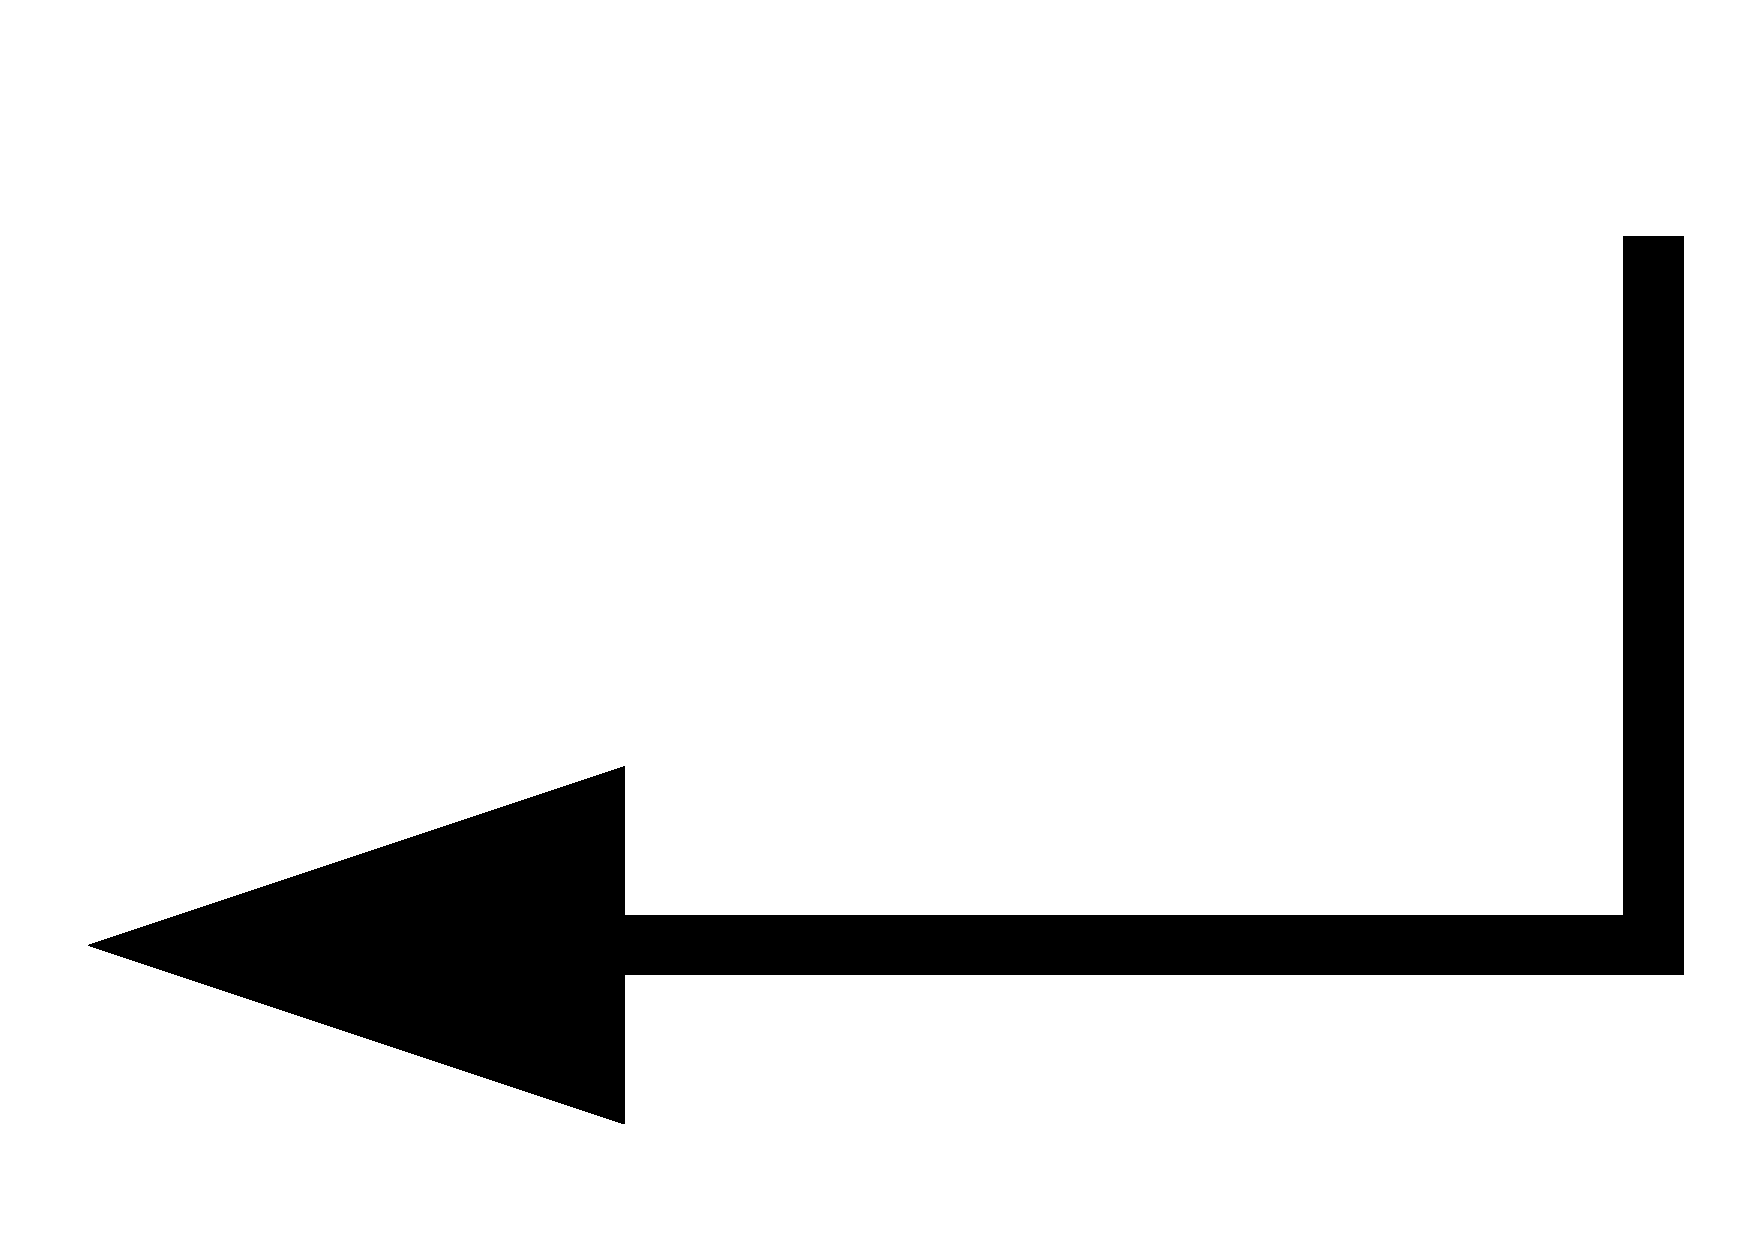
\includegraphics[width=1em]{images/return-symbol}}}

%% Change how subfigures are labelled
\makeatletter
\renewcommand{\@thesubfigure}{\figurename~\thefigure\alph{subfigure}: }
\renewcommand{\thesubfigure}{\alph{subfigure}}
%%%\renewcommand{\p@subfigure}{\alph{subfigure}}
\makeatother

% No indents at start of paragraph, but paragraphs have blank lines
% between them
\setlength{\parindent}{0pt}
\setlength{\parskip}{2ex} 


%% \filename allows for _ but otherwise is formatted identically to
%% code. If using tildes (~) then use \mytilde command, inside
%% \texttt. Use the url package's command to define this, that way
%% hyperref doesn't see it as a hyperref!
\DeclareUrlCommand\filename{\urlstyle{tt}}
\newcommand{\email}[1]{\href{mailto:#1}{#1}}
\newcommand{\ccThreeUrl}{http://creativecommons.org/licenses/by-sa/3.0/}

%% Environment variables. Like \filename but prepends a $
\DeclareUrlCommand\envVar{\def\UrlLeft{\$}\urlstyle{tt}}
\DeclareUrlCommand\dosEnvVar{\def\UrlLeft{\%}\def\UrlRight{\%}\urlstyle{tt}}

\newcommand{\code}[1]{\texttt{#1}}
\newcommand{\username}[1]{\texttt{#1}}
\newcommand{\piUser}{\username{pi}}
\newcommand{\rootUser}{\username{root}}

%% Use for menu selections etc
\newcommand{\myquote}[1]{\textcolor{MyQuoteColor}{\textsl{#1}}}

%% Define our own keypress command, based on keystroke
\newcommand{\keypress}[1]{\keystroke{#1}}

%% Units
%%\newcommand{\units}[2]{\mbox{\ensuremath{#1}\,#2}}
%%\newcommand{\dB}[1]{\mbox{\ensuremath{#1}\,dB}}
\newcommand{\dB}[1]{\SI{#1}{dB}}
\newcommand{\inch}[1]{\mbox{\ensuremath{#1}''}}
% \newcommand{\kHz}[1]{\mbox{\ensuremath{#1}\,kHz}}
%\newcommand{\metre}[1]{\mbox{\ensuremath{#1}\,m}}
\newcommand{\km}[1]{\mbox{\ensuremath{#1}\,km}}
%% \newcommand{\MHz}[1]{\mbox{\ensuremath{#1}\,MHz}}
\newcommand{\Hz}[1]{\SI{#1}{\hertz}}
\newcommand{\kHz}[1]{\SI{#1}{\kilo\hertz}}
\newcommand{\MHz}[1]{\SI{#1}{\mega\hertz}}
\newcommand{\volt}[1]{\mbox{\ensuremath{#1}\,V}}
\newcommand{\bit}[1]{\mbox{\ensuremath{#1}\,bit}}

%%\newcommand{\degrees}[1]{\ensuremath{#1^\circ}}

\renewcommand{\textohm}{\ensuremath{\Omega}}
\newcommand{\ohm}[1]{\SI{#1}{\ohm}}
\newcommand{\kohm}[1]{\SI{#1}{\kilo\ohm}}


\newcommand{\pF}[1]{\SI{#1}{\pico\farad}}
\newcommand{\nF}[1]{\SI{#1}{\nano\farad}}
\newcommand{\uF}[1]{\SI{#1}{\micro\farad}}

\newcommand{\uH}[1]{\SI{#1}{\micro\henry}}

%% Some simple abbreviations  
\newcommand{\ie}{i.e.}
\newcommand{\eg}{e.g.}
\newcommand{\etal}{\latin{et al.}}
\newcommand{\etc}{etc.}

%% Have warnings printed in light red box, with each item using a
%% STOP sign as a bullet
\newenvironment{warninglist}{%
  \begin{list}{\Stopsign}{}}{%
    \end{list}}
\newcommand{\warningbox}[1]{\noindent%
  \colorbox{MyLightRed}{\parbox{\textwidth}{%
      \begin{warninglist}\item #1\end{warninglist}}} \newline}

%% Have help information printed in light blue box, with each item using an
%% information sign as a bullet
\newenvironment{helplist}{%
  \begin{list}{\Info}{}}{%
    \end{list}}
\newcommand{\helpbox}[1]{\noindent
  \colorbox{MyLightBlue}{\parbox[l]{\textwidth}{%
      \begin{helplist}\item #1\end{helplist}}} \newline}

%% Verbatim-like environment for code.
\DefineVerbatimEnvironment{Code}{Verbatim}%
{frame=single,commandchars=\\\{\}}
\DefineVerbatimEnvironment{Cmd}{Verbatim}%
{frame=single,framesep=5mm,commandchars=\\\{\}}
% {frame=single,label=\linuxLogo,framesep=5mm,commandchars=\\\{\}}
\DefineVerbatimEnvironment{LinuxCmd}{Verbatim}%
{frame=single,framesep=5mm,commandchars=\\\{\}}
% {frame=single,label=\linuxLogo,framesep=5mm,commandchars=\\\{\}}
\DefineVerbatimEnvironment{WindowsCmd}{Verbatim}%
{frame=single,framesep=5mm,commandchars=\\\{\}}
% {frame=single,label=\windowsLogo,framesep=5mm,commandchars=\\\{\}}

%% \DefineVerbatimEnvironment{Cmd}{LinuxCmd}{}


\DefineVerbatimEnvironment{RootCmd}{Verbatim}%
{frame=single,framesep=5mm,label=As user \rootUser,commandchars=\\\{\}}
\DefineVerbatimEnvironment{PiCmd}{Verbatim}%
{frame=single,framesep=5mm,label=As user \piUser,commandchars=\\\{\}}


\newcommand{\todo}[1][]{\fcolorbox{magenta}{MyLightMagenta}{\mbox{\textcolor{black}{TO DO\ifthenelse{\equal{#1}{}}{}{: #1}}}}}

\newcommand{\figscale}{1.0}

%% Have subsubsections numbered
\setcounter{secnumdepth}{5}
\setcounter{tocdepth}{5}


\newenvironment{buildorder}{%
  \begin{enumerate}%
    \setlength{\itemsep}{0pt}%
    \setlength{\parskip}{0pt}}%
  {\end{enumerate}}

\newcommand{\documentAttribution}{``AuroraWatchNet magnetometer manual. Steve Marple, Lancaster
  University. 2013.''} 

\begin{document}

\title{AuroraWatchNet magnetometer manual}
\author{Steve Marple, \\
Lancaster University.}
\date{\today}
\maketitle
\thispagestyle{empty}
\frontmatter
\pagestyle{headings}

% \clearpage  
% \phantomsection  
% % \thispagestyle{empty}
\chapter{Licence}
This document is made available under the \href{\ccThreeUrl}{Creative
  Commons Attribution-ShareAlike 3.0 Unported Licence}.

\begin{center}
\href{\ccThreeUrl}{
\includegraphics{images/by-sa}}
\end{center}

Please attribute this work as \documentAttribution

\clearpage  
\phantomsection  
\addcontentsline{toc}{chapter}{\contentsname}  
\tableofcontents

\newpage
\phantomsection  
\addcontentsline{toc}{chapter}{\listfigurename}  
\listoffigures

%% -----------------------------
% \newpage
% \phantomsection  
% \addcontentsline{toc}{chapter}{\listtablename}  
% \listoftables

\newpage
\phantomsection  
\printabbrev

\mainmatter
%% Allow for sloppy wordbreaking to avoid text spilling into the
%% margin (eg as a result of \filename and other non-breaking text)
\sloppy
\part{Introduction}
\chapter{Overview of the hardware}

\section{Introduction}
The magnetometer is designed for low-power operation, simple
installation and ease of construction. The entire design is open
source, allowing anyone with reasonable soldering ability to construct
one.

The magnetometer has two major parts, the base unit and the sensor
unit (\figurename~\ref{fig:system-overview}). The sensor unit is located
outdoors, away from buildings, cars and other sources of human
disturbance. It is battery powered and communicates with the base unit
by a radio link (\MHz{433} or \MHz{868}), enabling the sensor to be
installed without any wiring to the base unit. The base unit is placed
indoors and should be positioned such that there are the minimum
number of walls between it and the sensor unit.

\begin{figure}
  \centering
  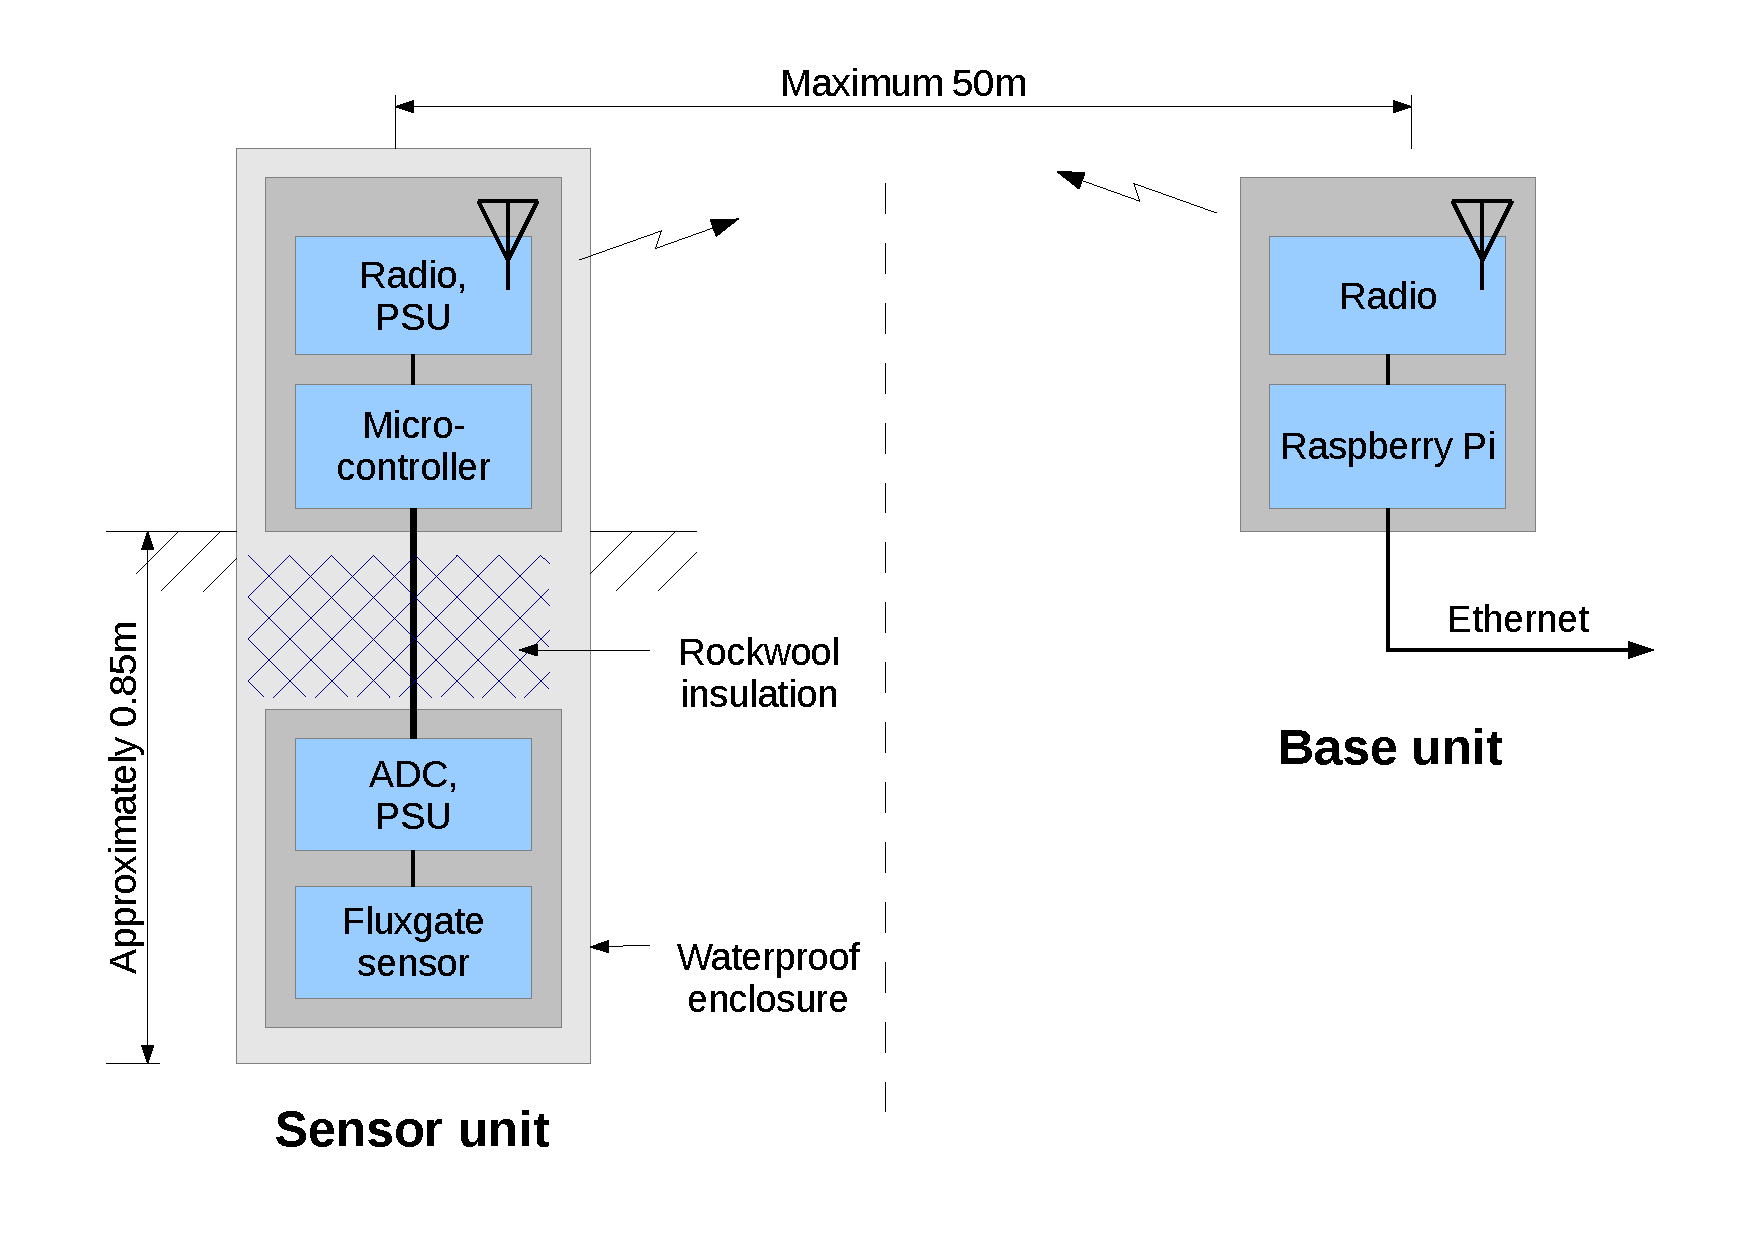
\includegraphics[keepaspectratio,width=\textwidth]{%
    calunium-mag/images/system-overview}
  \caption[System overview]%
  {System overview.}
  \label{fig:system-overview}
\end{figure}

\section{Sensor unit}

The sensor unit (figure~\ref{fig:sensor-unit}) is contained inside a
waterproof enclosure approximately \SI{1.1}{\metre} high which is
partially buried to reduce temperature variations and to provide a
stable foundation. The sensor itself is placed at the bottom of the
enclosure, approximately \SI{0.85}{\metre} below ground. The
microcontroller, radio module and battery are positioned in the top
part of the enclosure, above ground level. Insulating material (\eg\
rockwool) is used to fill the space in-between.

The
\href{http://blog.stevemarple.co.uk/search/label/Calunium}{Calunium}
microcontroller board is based on the popular
\href{http://arduino.cc}{Arduino} platform but uses the more powerful
Atmel ATmega1284P microcontroller.

\begin{figure}[!h]
  \centering
  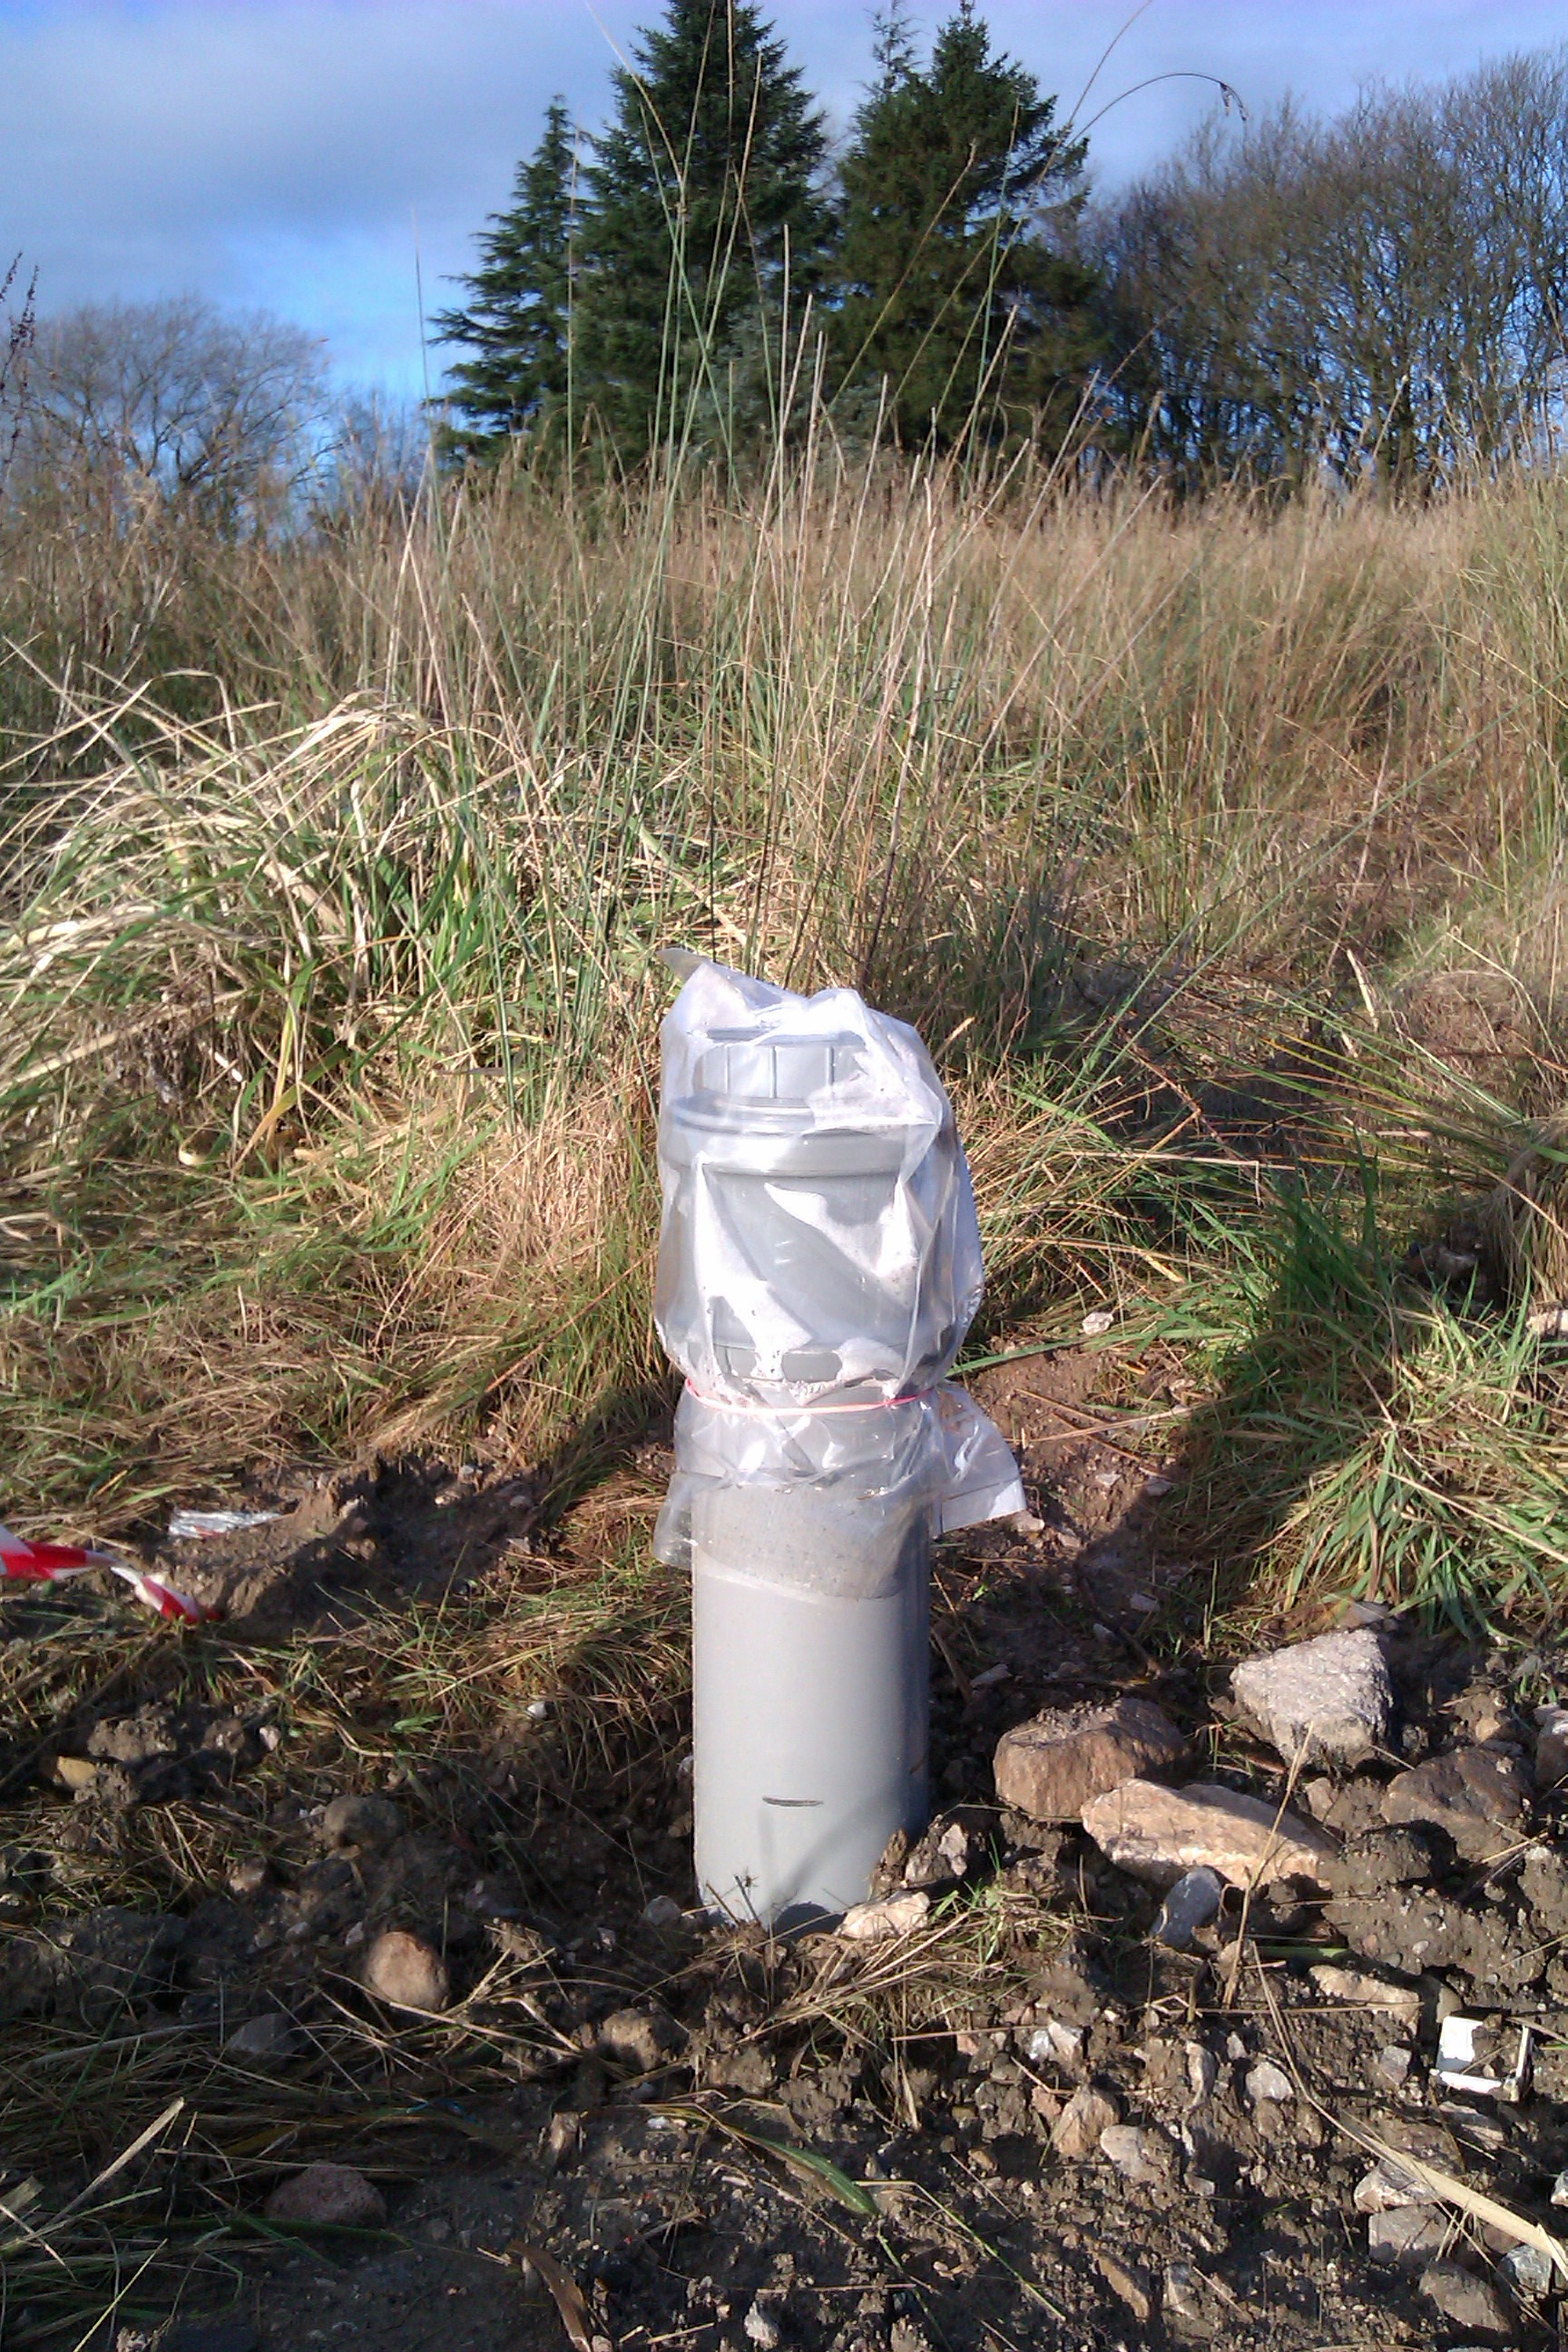
\includegraphics[keepaspectratio,height=10cm]{images/sensor-unit}
  \caption[Sensor unit]{%
    Sensor unit. \photoCredit{Steve Marple}{\ccBySaTwo}{%
      http://www.flickr.com/photos/stevemarple/8499204572/} 
  }
  \label{fig:sensor-unit}
\end{figure}

\begin{figure}
  \centering
  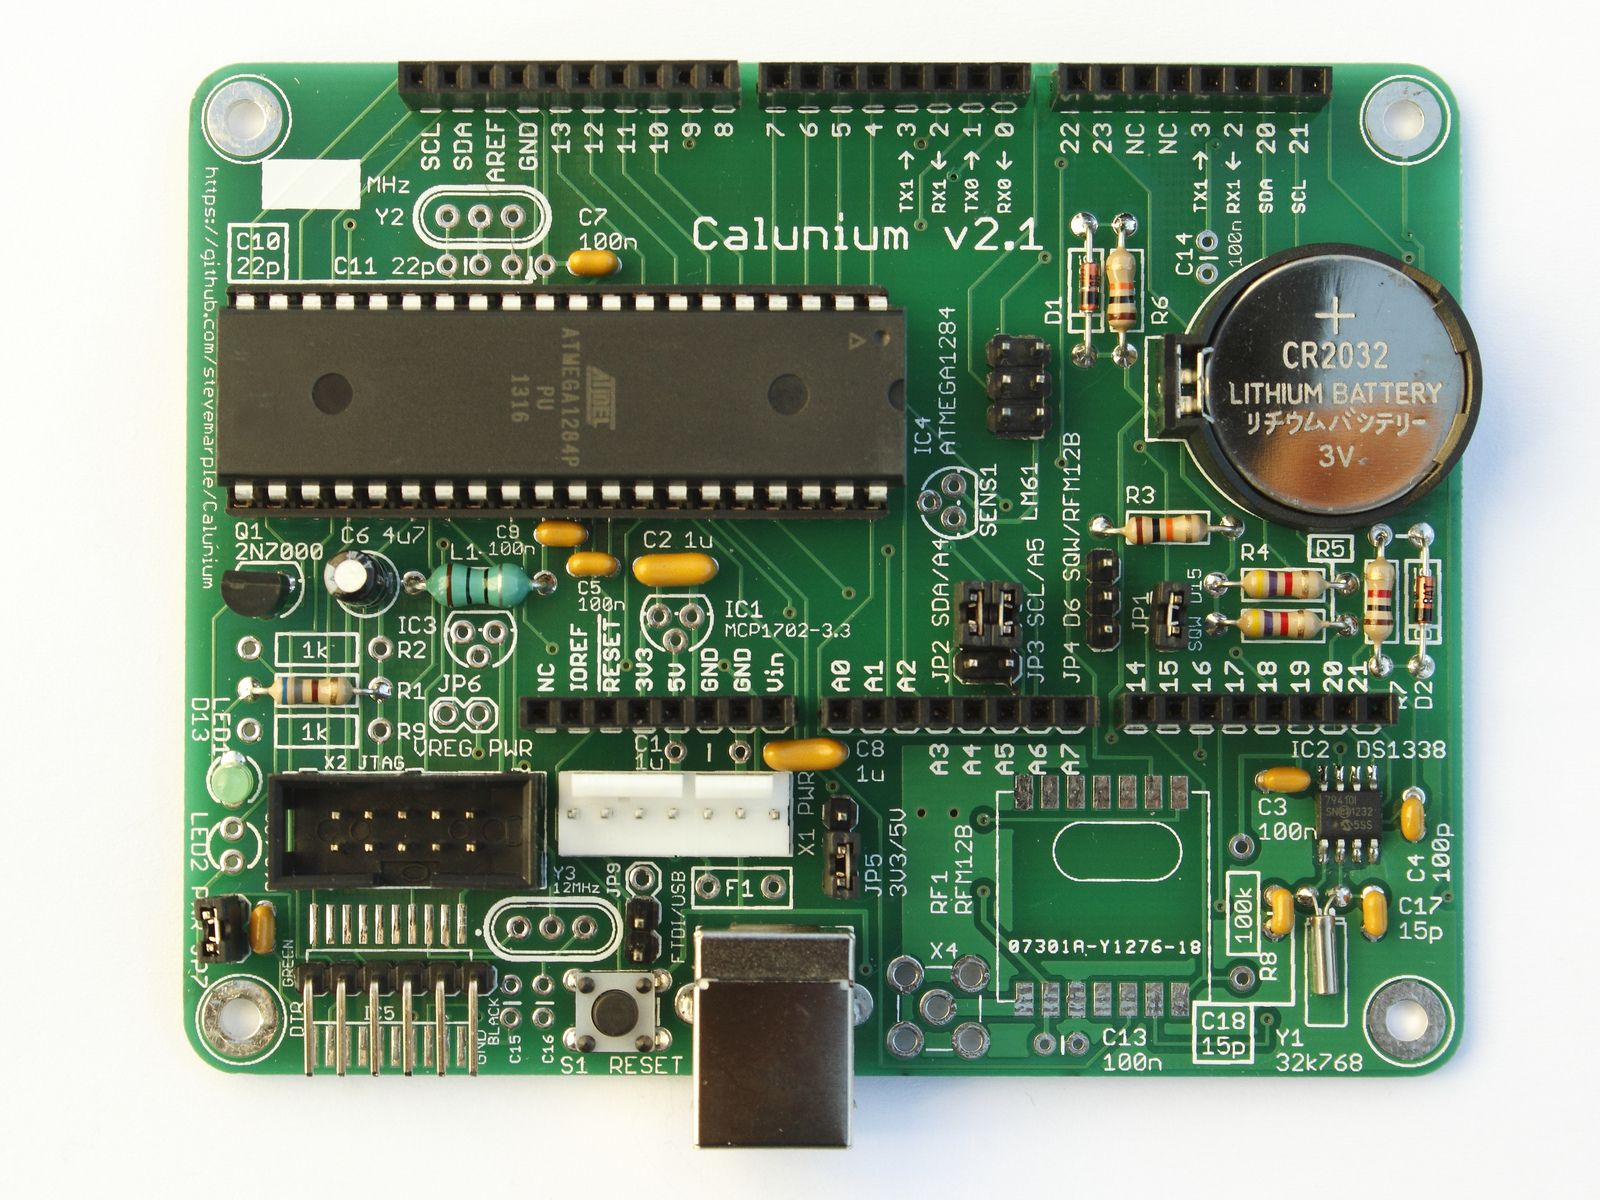
\includegraphics[keepaspectratio,width=\textwidth]{%
    images/calunium-v2-1}
  \caption[Calunium microcontroller PCB]{%
    Calunium microcontroller \pcb. %
    \photoCredit{Steve Marple}{\ccBySaTwo}{%
      http://www.flickr.com/photos/stevemarple/10786865096/}}
  \label{fig:calunium}
\end{figure}

\begin{figure}
  \centering
  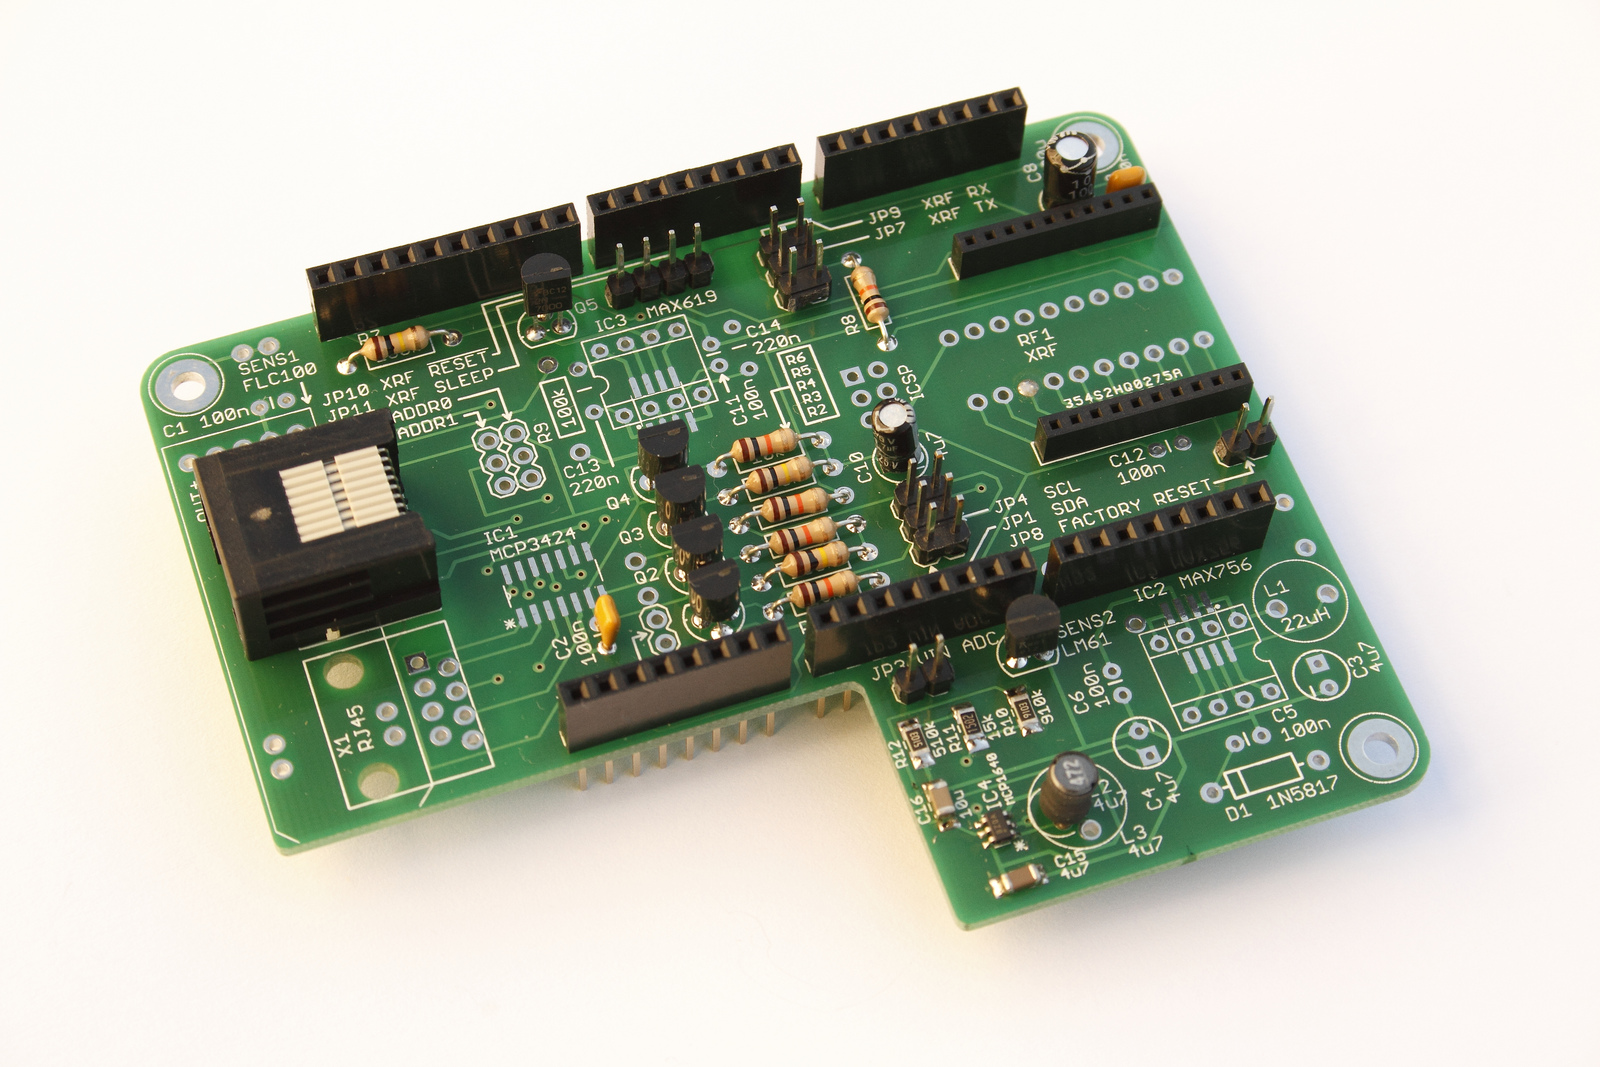
\includegraphics[keepaspectratio,width=\textwidth]{%
    images/flc100-shield}
  \caption[FLC100 shield]{The FLC100 shield fits onto the Calunium
    microcontroller \pcb. \photoCredit{Steve Marple}{\ccBySaTwo}{%
      http://www.flickr.com/photos/stevemarple/10787109594/}}
  \label{fig:flc-100-shield}
\end{figure}

\begin{figure}
  \centering
  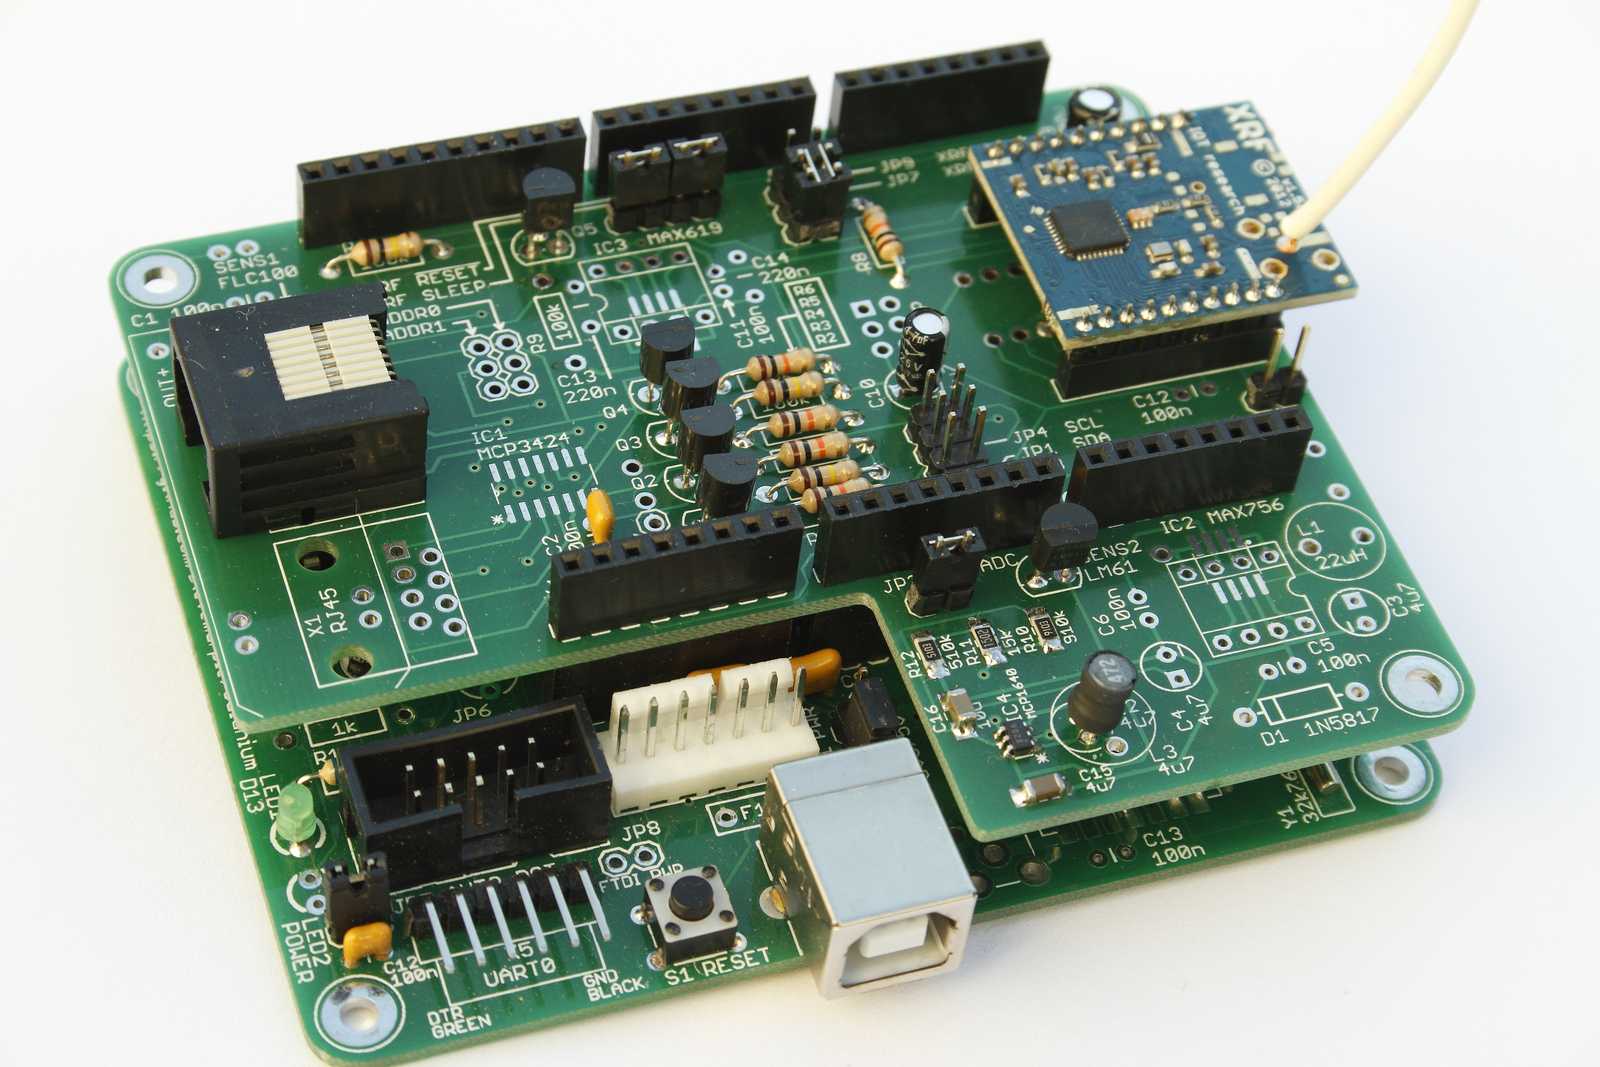
\includegraphics[keepaspectratio,width=\textwidth]{%
    images/calunium-flc100-shield.jpg}
  \caption[Calunium microcontroller board and FCL100 shield]{%
    Calunium microcontroller board and FCL100 shield. 
    \photoCredit{Steve Marple}{\ccBySaTwo}{%
      http://www.flickr.com/photos/stevemarple/10913562526/}}
  \label{fig:calunium-flc-100-shield}
\end{figure}

\clearpage
\section{Base unit}

The base unit is a \href{http://www.raspberrypi.org/‎}{Raspberry Pi}
single-board computer with a radio transceiver unit. The Ethernet
interface of the Raspberry Pi is used to send the magnetic field
measurements to AuroraWatch UK. When the Raspberry Pi is accessed over
the network with Secure Shell (\ssh) a display and keyboard are not
needed. The Raspberry Pi runs the Raspbian linux distribution. The
receiving software is written in Python.

\begin{figure}[!h]
  \centering
  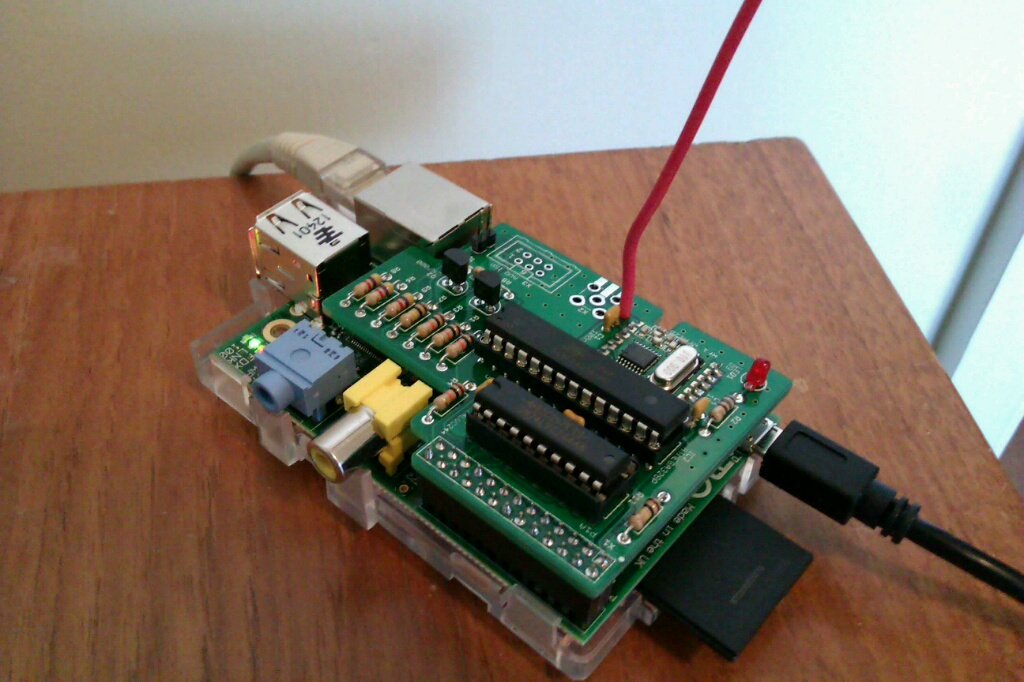
\includegraphics[keepaspectratio,height=10cm]{images/base-unit}
  \caption[Base unit]{%
    Base unit. \photoCredit{Steve Marple}{\ccBySaTwo}{%
      http://www.flickr.com/photos/stevemarple/10787215844/}}
  \label{fig:base-unit}
\end{figure}


\part{Construction}
\chapter{Beginning construction}

\section{Anti-static precautions}

\section{Tools required}

\begin{itemize}
\item Soldering iron.
\item Sidecutters.
\item Small pliers.
\item In-circuit serial programmer for Atmel AVR microcontrollers,
  \eg, \href{http://www.atmel.com/tools/AVRDRAGON.aspx}{Atmel AVR Dragon}.
\item \usb\ to \ttl\ serial converter for \volt{3.3} operation, \eg, FTDI
  TTL-232R-3V3.
\item Digital multimeter.
\item Solderless breadboard (optional).
\end{itemize}

\section{Order of assembly}

For ease of access components should normally be fitted in order of
increasing size, particularly increasing height. If this order is not
observed it can ver very difficult to access the pads of surface mount
devies. It is also preferable that \emph{passive} components
(resistors, capacitors, inductors and crystals) are fitted before
semiconductors (field-effect transistors, integreated circuits). This
is because the semiconductors are easily damaged by electro-static
discharge (sometimes this damage isn't immediately obvious). It is
therefore more convenient to fit as many components as possible before
fitting the semiconductors, at which point \esd\ precautions should be
followed. As field-effect transistors are particularly vulnerable to
damage by \esd\ it is recommended they are fitted as late as possible.
From these guidelines the following order is recommended.
\begin{itemize}
\item Surface-mount passive components.
\item Surface-mount semiconductors.
\item Through-hole passive components.
\item Through-hole semiconductors (\fet s last).
\item Switches.
\item Connectors, battery holders.
\end{itemize}

The first \pcb\ to be assembled is the FLC100 shield, this board
provides the power to the system and will enable you to test each part
correctly.

\chapter{FLC100 shield assembly}

\section{Introduction}
The FLC100 shield is an Arduino ``shield'' which interfaces the
microcontroller to the FLC100 fluxgate magnetometer sensor, if
necessary translating logic levels. It is also responsible for
generating the correct operating voltage for the
microcontroller. There is more than one version of this board, be sure
to use the instructions appropriate to your version.

\section{FLC100 shield version 1.0}

\subsection{Description}

The FLC100 shield version 1.0 operates at \volt{3.3}. \textbf{Do not
  attempt to use it with standard Arduino boards which are operated at
  \volt{5}.} The shield houses the XRF radio module, the boost power
supply (which creates the \volt{3.3} supply for the microcontroller
and radio) and the \volt{3.3} -- \volt{5} level shifters.

There are both through-hole and surface mount versions of the boost
power supply. It is suspected that the through-hole version causes
\rfi\ since the radio module often fails to receive messages. This
problem was not apparent on the prototype board. The surface-mount
version has no such problems and is the option which should be
used. It is also cheaper and more efficient.

There is an option to fit a FLC100 sensor directly to the circuit
board. This option is not used because the FLC100 is slightly
temperature sensitive and better performance is obtained by
positioning the sensor below ground. Whilst the board provides an
option to fit an MCP3424 \adc\ and MAX619 charge-pump power supply they
are also fitted remotely, below ground, for reasons of temperature
stability.


\begin{figure}
  \centering
  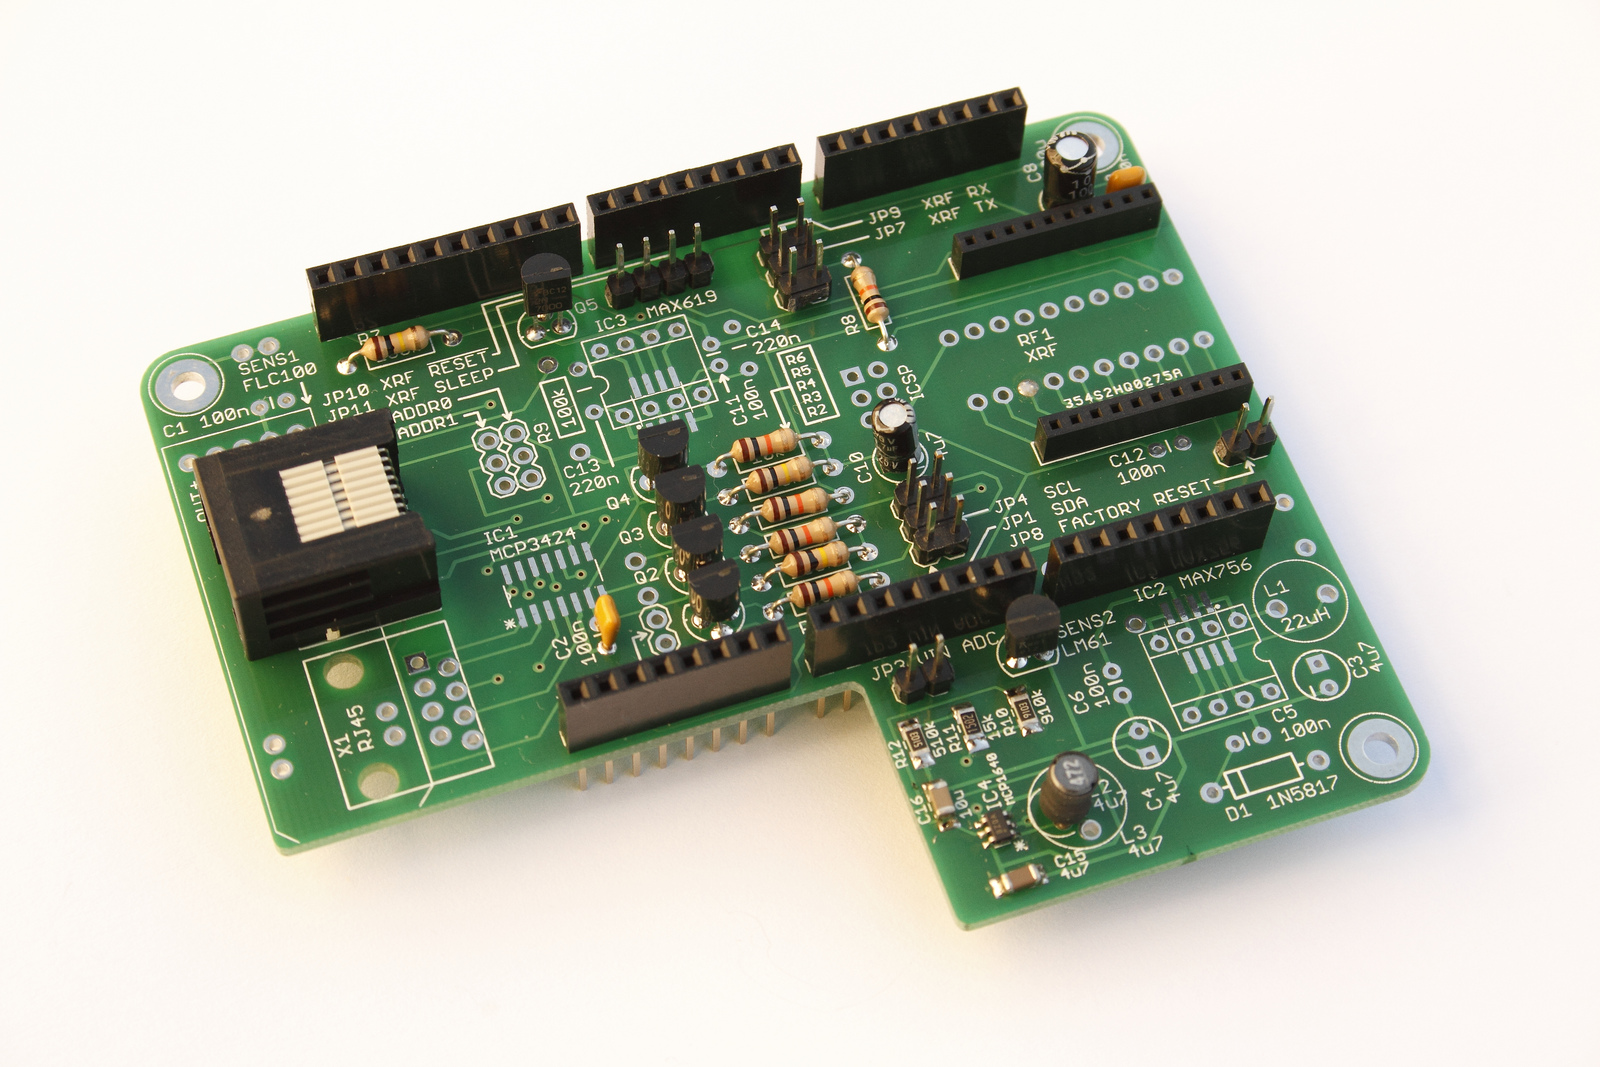
\includegraphics[keepaspectratio,width=\textwidth]{%
    images/flc100-shield}
  \caption[Completed FLC100 shield]{Completed FLC100 shield, except
    for fitting shunts onto the jumpers. %
    \photoCredit{Steve Marple}{\ccBySaTwo}{%
      http://www.flickr.com/photos/stevemarple/10787109594/}}
  \label{fig:flc100-v1.0}
\end{figure}

\subsection{Order of assembly}
\begin{buildorder}
\item IC4 (MCP1640).
\item R12 (\kohm{510}).
\item R11 (\kohm{15}).
\item R10 (\kohm{910}).
\item C15 (\uF{4.7}).
\item C16 (\uF{10}).
\item \SI{2}{\milli\metre} 10~way connectors for RF1. Ensure they are
  fitted flush to the \pcb.
\item R1, R3, R4, R6, R8 (\kohm{10}).
\item R2, R5, R7 (\kohm{100}).
\item C2, C7, C9 (\nF{100}).
\item C10 (\uF{4.7}).
\item C8 (\uF{100}).
\item L2 (\uH{4.7}). The shorter lead should be connected to pin~1,
  which is the hole nearest the edge of the \pcb. Although the
  orientation of inductors is normally ignored communication with the
  manufacturer revealed that the shorter lead indicates the start of
  the winding. This arrangement is preferred to help minimise \rfi.
\item Stacking connectors, five 8~way and one 10~way. Ensure they are
  fitted flush to the \pcb; solder one end first, then the other
  end. Only when you are happy they are flush should you solder the
  remaining pins.
\item JP1, JP4 ($2 \times 3$ jumper).
\item JP7, JP9 ($2 \times 3$ jumper).
\item JP10, JP11 ($1 \times 4$ jumper).
\item JP3 ($1 \times 2$ jumper).
\item JP8 ($1 \times 2$ jumper).
\item X2 (RJ45 connector).
\item Modify the \pcb\ by adding a link wire from the XRF ONSLEEP
  status pin to D23. See figure~\ref{fig:flc100-sleep-status-mod}.
\item Q1, Q2, Q3, Q4, Q5 (2N7000).
\end{buildorder}

\begin{figure}
  \centering
  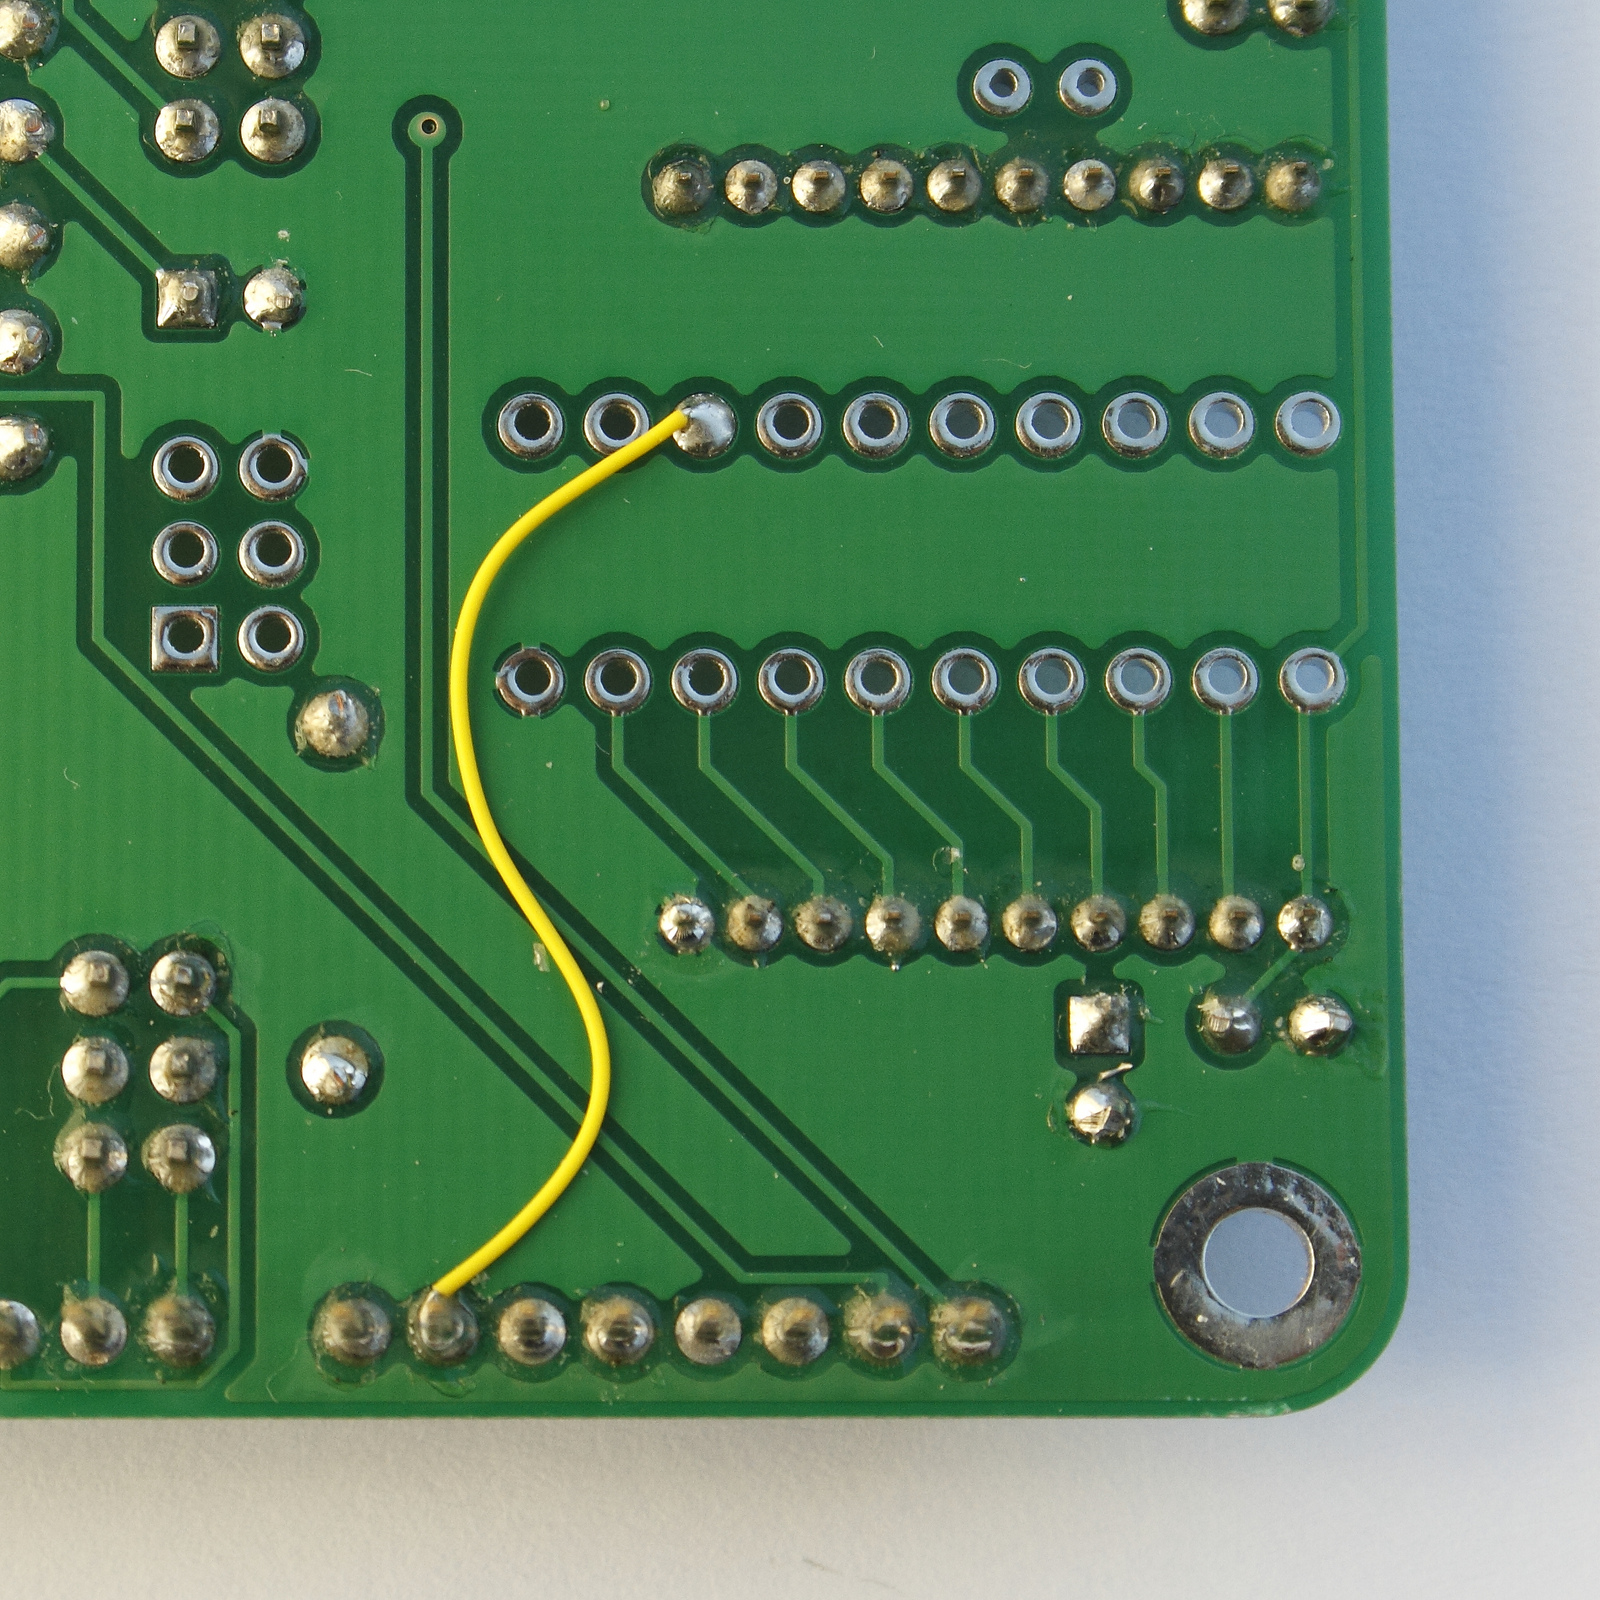
\includegraphics[keepaspectratio,width=10cm]{%
    images/flc100-sleep-status-mod}
  \caption[Modification to monitor sleep status of the XRF radio module]{%
    Modification to monitor sleep status of the XRF radio module.
    \photoCredit{Steve Marple}{\ccBySaTwo}{%
      http://www.flickr.com/photos/stevemarple/10786910376/}}
  \label{fig:flc100-sleep-status-mod}
\end{figure}


Fit shunts to JP10, JP11, JP3. Fit shunts to JP7 and JP9, to the two
connectors furthest from the edge of the \pcb. \textbf{Do not fit the
  shunts so that they bridge between JP7 and JP9}.

If the microcontroller board has dedicated \itwoc\ connections (\eg
Calunium v2.0 or later), then no shunts should be fitted to JP1 and
JP4. If the microcontroller has \itwoc\ connections in the standard
Arduino Mega positions (\eg, Calunium v1.0, Arduino Mega, Arduino Mega
2560) then fit shunts to JP1 and JP4 to the two connectors closest to
C10, otherwise fit shunts to JP1 and JP4 to the two connectors closest
to the stacking connectors. \textbf{In no circumstances should the
  shunts bridge between JP1 and JP4}.

Leave JP8 open circuit. It is fitted only when the XRF1 radio module
must be forced to use the default factory configuration.

\begin{landscape}
  \begin{figure}[p]
    \centering
    \includegraphics[keepaspectratio,width=28cm,height=16cm]{%
      images/FLC100_shield_v1_0_sch}
    \caption{FLC100 shield v.~1.0 circuit diagram.}
    \label{fig:flc100-shield-v1.0-cct-diag}
  \end{figure}
\end{landscape}

\section{FLC100 shield version 2.0}

\subsection{Description}

The FLC100 shield version 2.0 can operate at either \volt{3.3} or
\volt{5}. This enables the board to be used either for battery-powered
systems, with the microcontroller and radio operating at \volt{3.3} or
with the standard Arduino Ethernet shield which requires the shield
and microcontroller to operate at \volt{5}. When used in conjunction
with the Arduino Ethernet shield it is assumed that the \PoE\ module
is fitted. The operating voltage chosen during construction determines
which components are fitted.

The shield can also be used for cloud detection, for which it supports
the operation of an MLX90614 non-contact \ir\ thermometer, HIH61xx
humidity and ambient temperature sensor, and Embedded Adeventures
lightning sensor module. These functions are outside of the scope of
this document and will not be described here.

\subsubsection{Battery operation}
When built for battery operation the shield houses the XRF radio
module, the boost power supply (which creates the \volt{3.3} supply
for the microcontroller and radio) and the \volt{3.3} -- \volt{5}
level shifters. The boost regulator can be built onto the \pcb\ using
discrete components. A simpler alternative which avoids the need to
solder small surface mount components is to fit a ready-built
third-party module.


\subsubsection{Power over ethernet operation}
If used in conjunction with the Ethernet shield the
XRF radio module and boost power supply are not fitted. The Ethernet
shield provides a \volt{9} output onto the \texttt{Vin} pin,
requiring that a linear or buck regulator is fitted for \volt{5} operation.

\subsection{Order of assembly}
\subsubsection{Battery-powered version}

\warningbox{Build instructions for the battery-powered option of the
  FLC100 shield version 2.0 are untested. Proceeed with caution.}

Order of assembly for the battery-powered version.

If using the on-board surface-mount boost regulator fit:
\begin{buildorder}
\item IC4 (MCP1640).
\item R19 (\kohm{510}).
\item R18 (\kohm{15}).
\item R17 (\kohm{910}).
\item C4 (\uF{4.7}).
\item C5 (\uF{10}).
\end{buildorder}

For all battery-powered versions fit:

\begin{buildorder*}
\item \SI{2}{\milli\metre} 10~way connectors for RF1. Ensure they are
  fitted flush to the \pcb.
\item R4 (\kohm{1}).
\item R1, R3, R5, R7, (\kohm{10}).
\item R2, R6 (\kohm{100}).
\item R8 (\Mohm{1}).
\item C1, C3 (\nF{100}).
\item C2, C9 (\uF{100}).
\item C6 (\uF{100} \volt{25}).
\item L1 (\uH{4.7}). The shorter lead should be connected to pin~1,
  which is the hole nearest the edge of the \pcb. Although the
  orientation of inductors is normally ignored communication with the
  manufacturer revealed that the shorter lead indicates the start of
  the winding. This arrangement is preferred to help minimise \rfi.
\item Stacking connectors, five 8~way and one 10~way. Ensure they are
  fitted flush to the \pcb; solder one end first, then the other
  end. Only when you are happy they are flush should you solder the
  remaining pins.
\item JP2 ($1 \times 2$ jumper).
\item JP3, JP5 ($1 \times 3$ jumper).
\item JP4, ISP header ($2 \times 3$ jumper).
\item X1 (RJ45 connector).
\item Q1, Q2, Q3, Q4, Q5 (2N7000). Fit last to minimise risk of damage
  from \esd.
\end{buildorder*}

If using an external boost regulator fit:
\begin{buildorder*}
\item Boost regulator module (Ciseco PowerPOD NCP1402 3V3).
\end{buildorder*}


\subsubsection[Order of assembly: PoE version]{%
  Order of assembly: \protect\PoE\ version}

\warningbox{Build instructions for \PoE\ option of the FLC100 shield
  version 2.0 are untested. Proceeed with caution.}  Order of assembly
for the \PoE\ version.
\begin{buildorder}
\item R1, R3, R5, R7, (\kohm{10}).
\item R2, R6 (\kohm{100}).
\item C1, C3 (\nF{100}).
\item C7 (\uF{4.7}).
\item C2, C9 (\uF{100}).
\item C6 (\uF{100} \volt{25}).
\item L1 (\uH{4.7}). The shorter lead should be connected to pin~1,
  which is the hole nearest the edge of the \pcb. Although the
  orientation of inductors is normally ignored communication with the
  manufacturer revealed that the shorter lead indicates the start of
  the winding. This arrangement is preferred to help minimise \rfi.
\item Stacking connectors, five 8~way and one 10~way. Ensure they are
  fitted flush to the \pcb; solder one end first, then the other
  end. Only when you are happy they are flush should you solder the
  remaining pins.
\item JP3 ($1 \times 3$ jumper).
\item JP4, ISP header ($2 \times 3$ jumper).
\end{buildorder}

If the master \pcb\ of the FLC100 remote sensor is version 2.0 and it
will be fitted with a linear regulator (MCP1702) then JP5 can be
omitted. Otherwise fit:
\begin{buildorder*}
\item JP5 ($1 \times 3$ jumper).
\item Add shunt to JP5, connect the centre pin to \texttt{Vin} if a
  linear regulator is fitted to the master FLC100 remote sensor \pcb;
  connect to \texttt{+3V3} if the MAX619 boost regulator is used on
  the master FLC100 remote sensor \pcb.
\end{buildorder*}


The connector to the remote sensor \pcb{}(s) can be either RJ11 or
RJ45. The RJ45 has the advantage that a standard (straight-through)
ethernet cable can be used. However it has the disadvantage that it is
possible to inadvertently fit the \PoE\ ethernet connection into the
wrong socket.
\begin{buildorder*}
\item X1 (RJ45 connector) or X2 (RJ11 connector). 
\end{buildorder*}

Add shunts to jumper blocks\marginpar{to complete}.
\begin{buildorder*}
\item Fit 3 shunts to JP4, in the positions marked on the silkscreen.
\item Fit a shunt to JP5, linking the centre pin with \texttt{+5V}.
\end{buildorder*}

\warningbox{If JP2 is fitted \textbf{do not} fit a shunt when used for
  \PoE\ operation, it will damage the microcontroller. Measurement of
  the input voltage can only be performed when $\textrm{V}_{\textrm{in}} \le
  \textrm{V}_{\textrm{cc}}$.}

Finally fit last to minimise risk of damage from \esd.
\begin{buildorder*}
\item Q1, Q2, Q3, Q4 (2N7000).
\end{buildorder*}


\subsubsection{Other variations}
If is possible (though not desirable) for the \volt{5} supply for the
remote sensor \pcb{}(s) to be generated by the FLC100 shield. To enable
this fit JP1 and add a shunt to link the \volt{5} rails between the
\pcb{}s.


\begin{landscape}
  \begin{figure}[p]
    \centering
    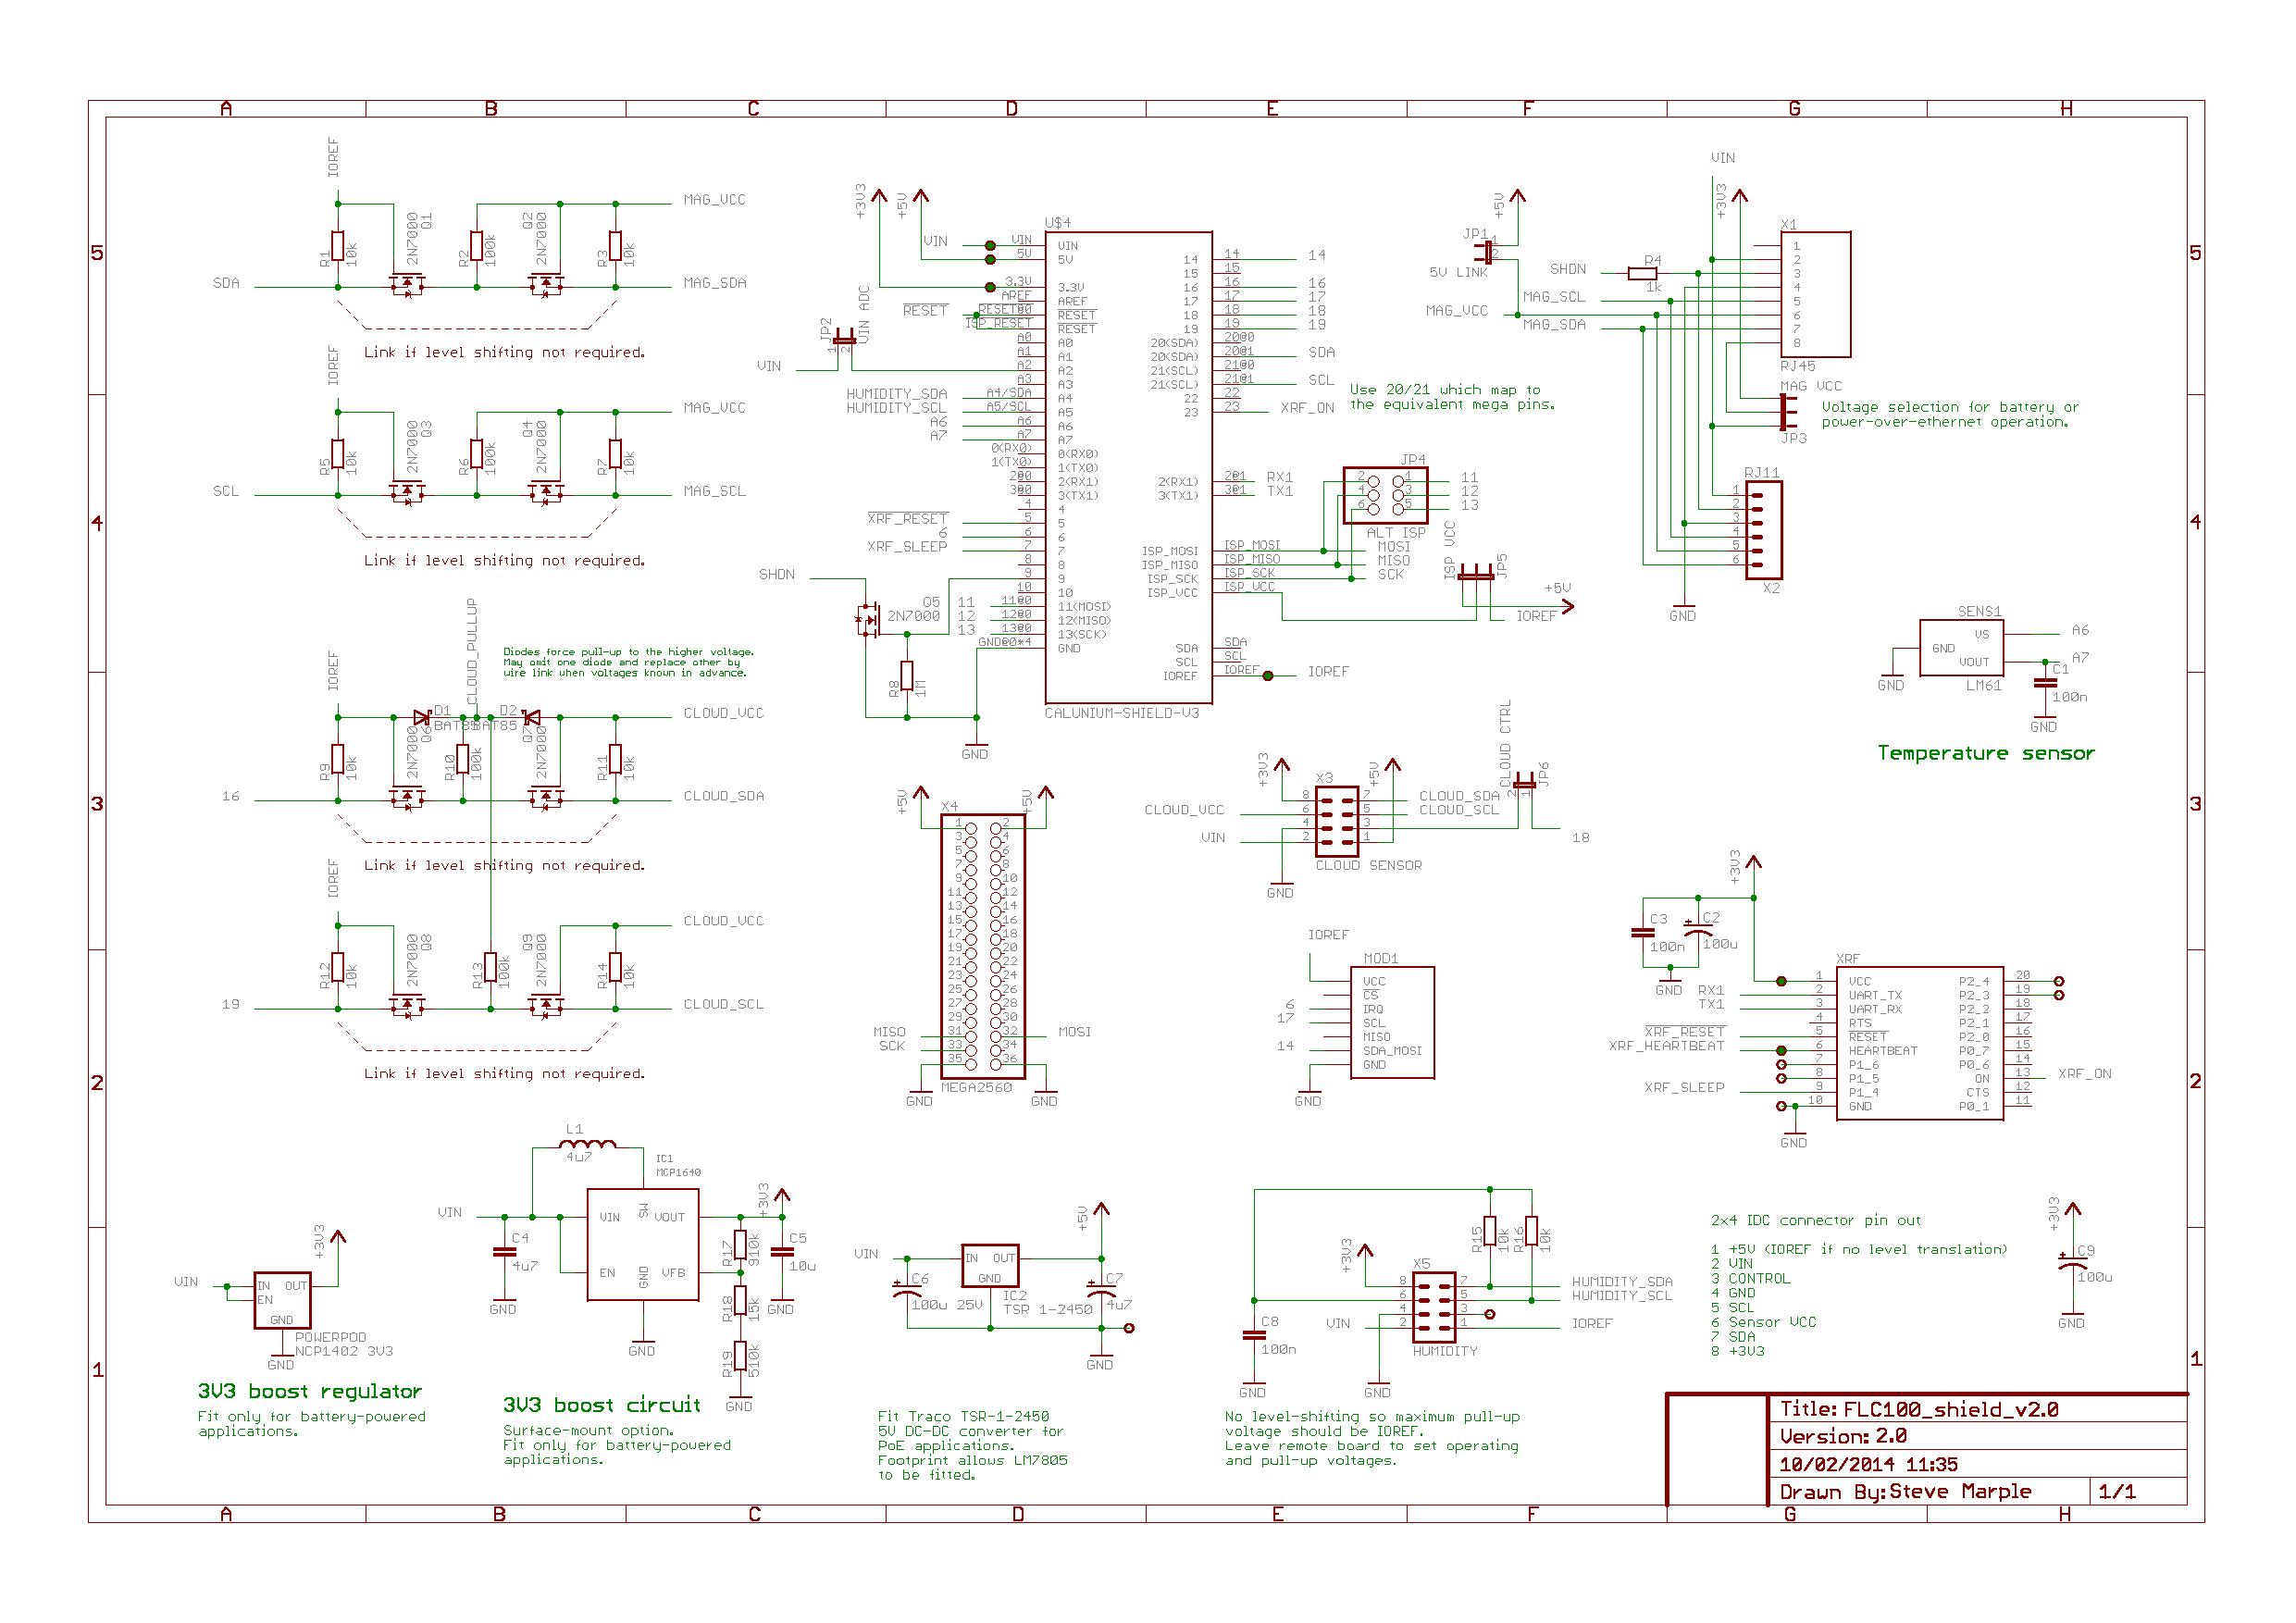
\includegraphics[keepaspectratio,width=28cm,height=16cm]{%
      images/FLC100_shield_v2_0_sch}
    \caption{FLC100 shield v.~2.0 circuit diagram.}
    \label{fig:flc100-shield-v2.0-cct-diag}
  \end{figure}
\end{landscape}

\chapter{Calunium assembly}

\section{Introduction}

The Calunium microcontroller development board is intended to be a
flexible system for both development and embedded use. As such it has
various hardware options and careful attention must be paid to
assembling it for optimum performance. Parts which are not needed are
omitted to lower power consumption (\eg, power LED, USB controller).

\section{Calunium version 2.0 and version 2.1}

\begin{figure}
  \centering
  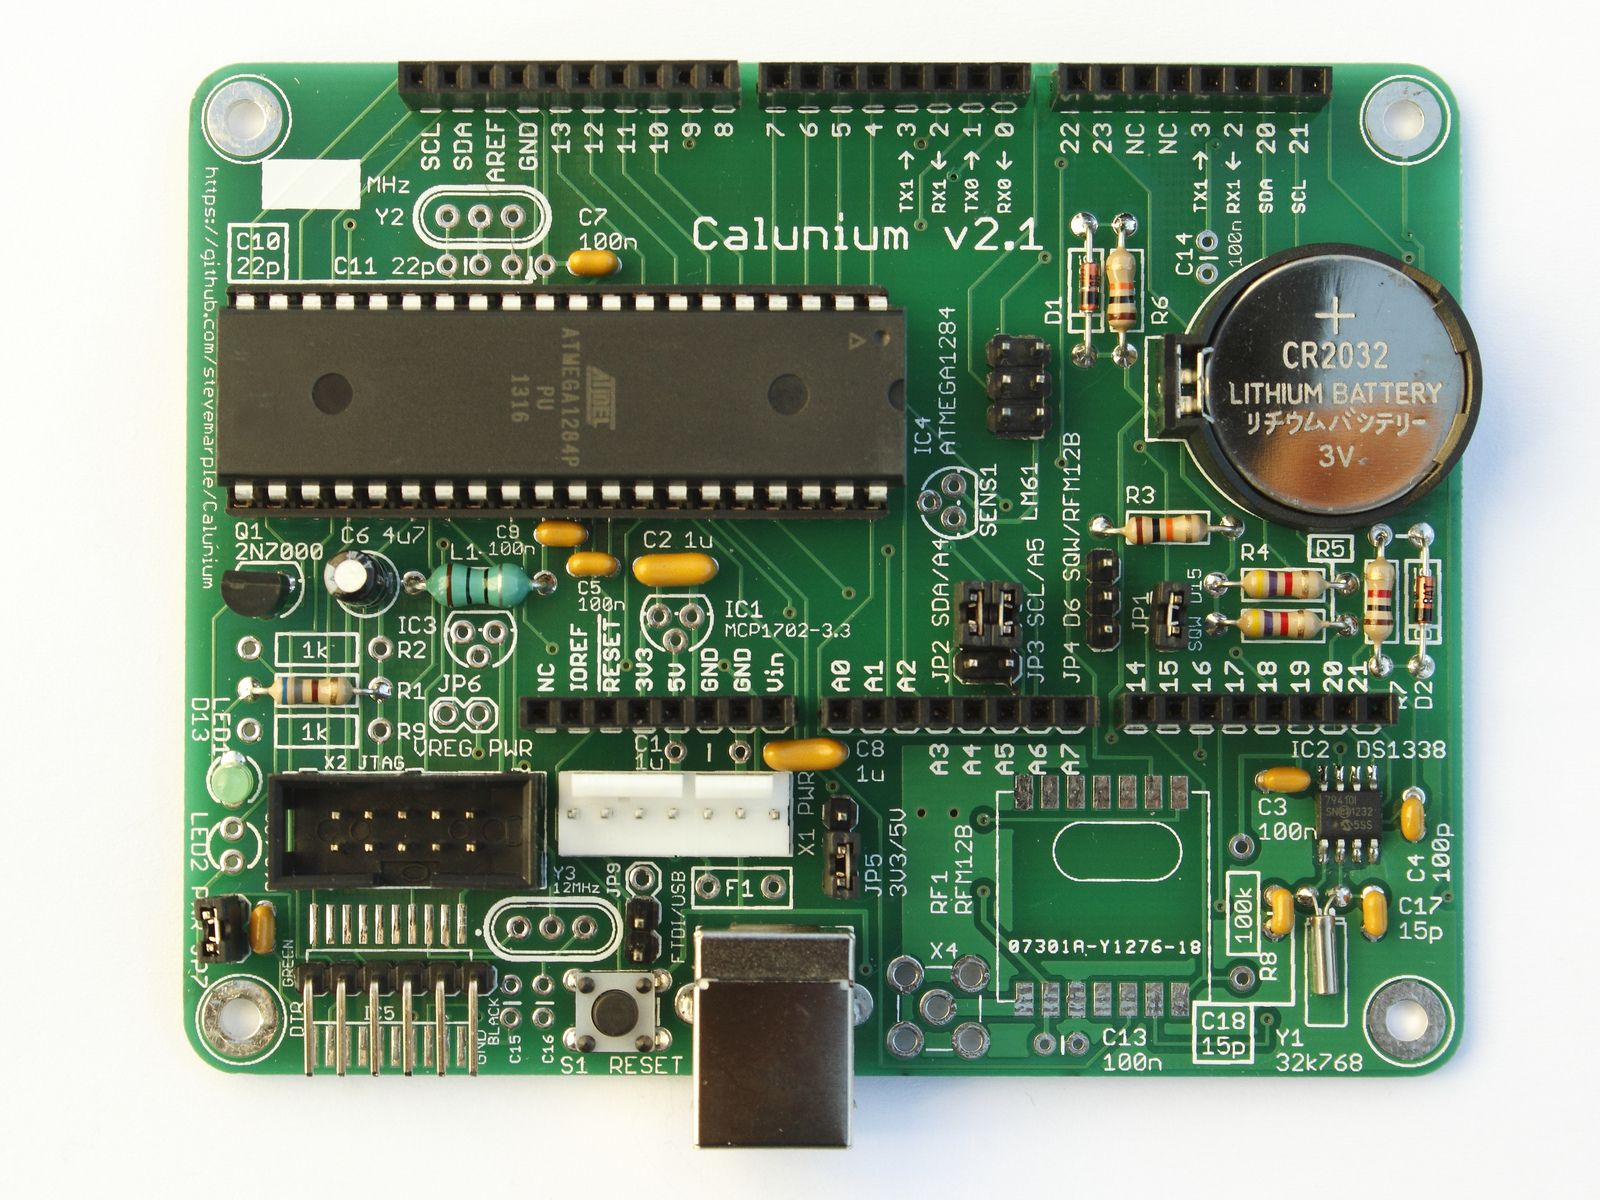
\includegraphics[keepaspectratio,width=\textwidth]{%
    images/calunium-v2-1}
  \caption[Completed Calunium v2.1]{%
    Completed Calunium v2.1. \photoCredit{Steve Marple}{\ccBySaTwo}{%
      http://www.flickr.com/photos/stevemarple/10786865096/}}
  \label{fig:calunium-version-2.1}
\end{figure}

\subsection{Order of assembly}

Fit components in order:
\begin{buildorder}
\item IC2. The standard real-time clock is the MicroChip MCP90410 but
  MicroChip MCP79411 or MCP79412 can be used without any other
  changes.
  It is also possible to fit the Maxim DS1338-33 real-time clock,
  but see below for changes.
\item Y1 (\kHz{32.768}).
\item R1, fit a \ohm{680} resistor. Ignore the \kohm{1} marking; a
  lower value resistor is used to enable the green LED to be seen
  more clearly in daylight.
\item R7 (\kohm{1}). Do not fit if using the DS1338-33 real-time
  clock. Instead link between R7 and D2 at the end nearest the \rtc\
  battery, as indicated by the white line on the silkscreen. The wire
  will bypass both R7 and D2 which are not required for the DS1338-33.
\item R4, R5 (\kohm{4.7}).
\item R3, R6 (\kohm{10}).
\item L1 (\uH{10}).
\item 40~pin socket for IC4.
\item C4 (\pF{100}).
\item C3, C5, C7, C9, C12 (\nF{100}).
\item C2, C8 (\uF{1}).
\item D1, D2 (BAT85). Do not fit D2 if using the DS1338-33 real-time clock.
\item LED1 (green LED). The cathode is nearest LED2, see
  figure~\ref{fig:calunium-led-orientation}.
\item C6 (\uF{4.7}).
\item ICSP header ($2 \times 3$ jumper block). See
  \figurename~\ref{fig:icsp-header}.
\item JP2 and JP3. Fit as combined $2 \times 3$ jumper block.
\item JP1, JP7 ($1 \times 2$ jumper).
\item JP4, JP5 ($1 \times 5$ jumper).
\item X5 ($1 \times 6$ right-angle or vertical header for UART0).
\item S1 (reset switch).
\item Arduino headers. \todo[Add description]
\item C17, C18 (\pF{15}). Do not fit if using DS1338-33 \rtc. For
  Calunium version 2.0 the capacitors must be fitted on the reverse
  side of the board (see \figurename~\ref{fig:calunium-rtc-caps-hack}
  as no specific mounting holes exist (error caused by using an
  earlier, incorrect datasheet which did not show the load
  capacitors).
\item X1 (Molex power header). Ensure correct orientation, with the
  backplate closest to the Arduino headers.
\item \todo[Add component name] (\rtc\ battery holder).
\item Q1 (2N7000). This item is very sensitive to damage by
  electrostatic discharge!
\item Battery (CR2032). Check that the battery backup pin (3) on the
  \rtc\ measures \volt{3.0}.
\item \todo[Fit shunts to jumpers \ldots]
\end{buildorder}
Do not fit the ATmega1284P microcontroller until after testing the
board power supplies.

\begin{figure}
  \centering
  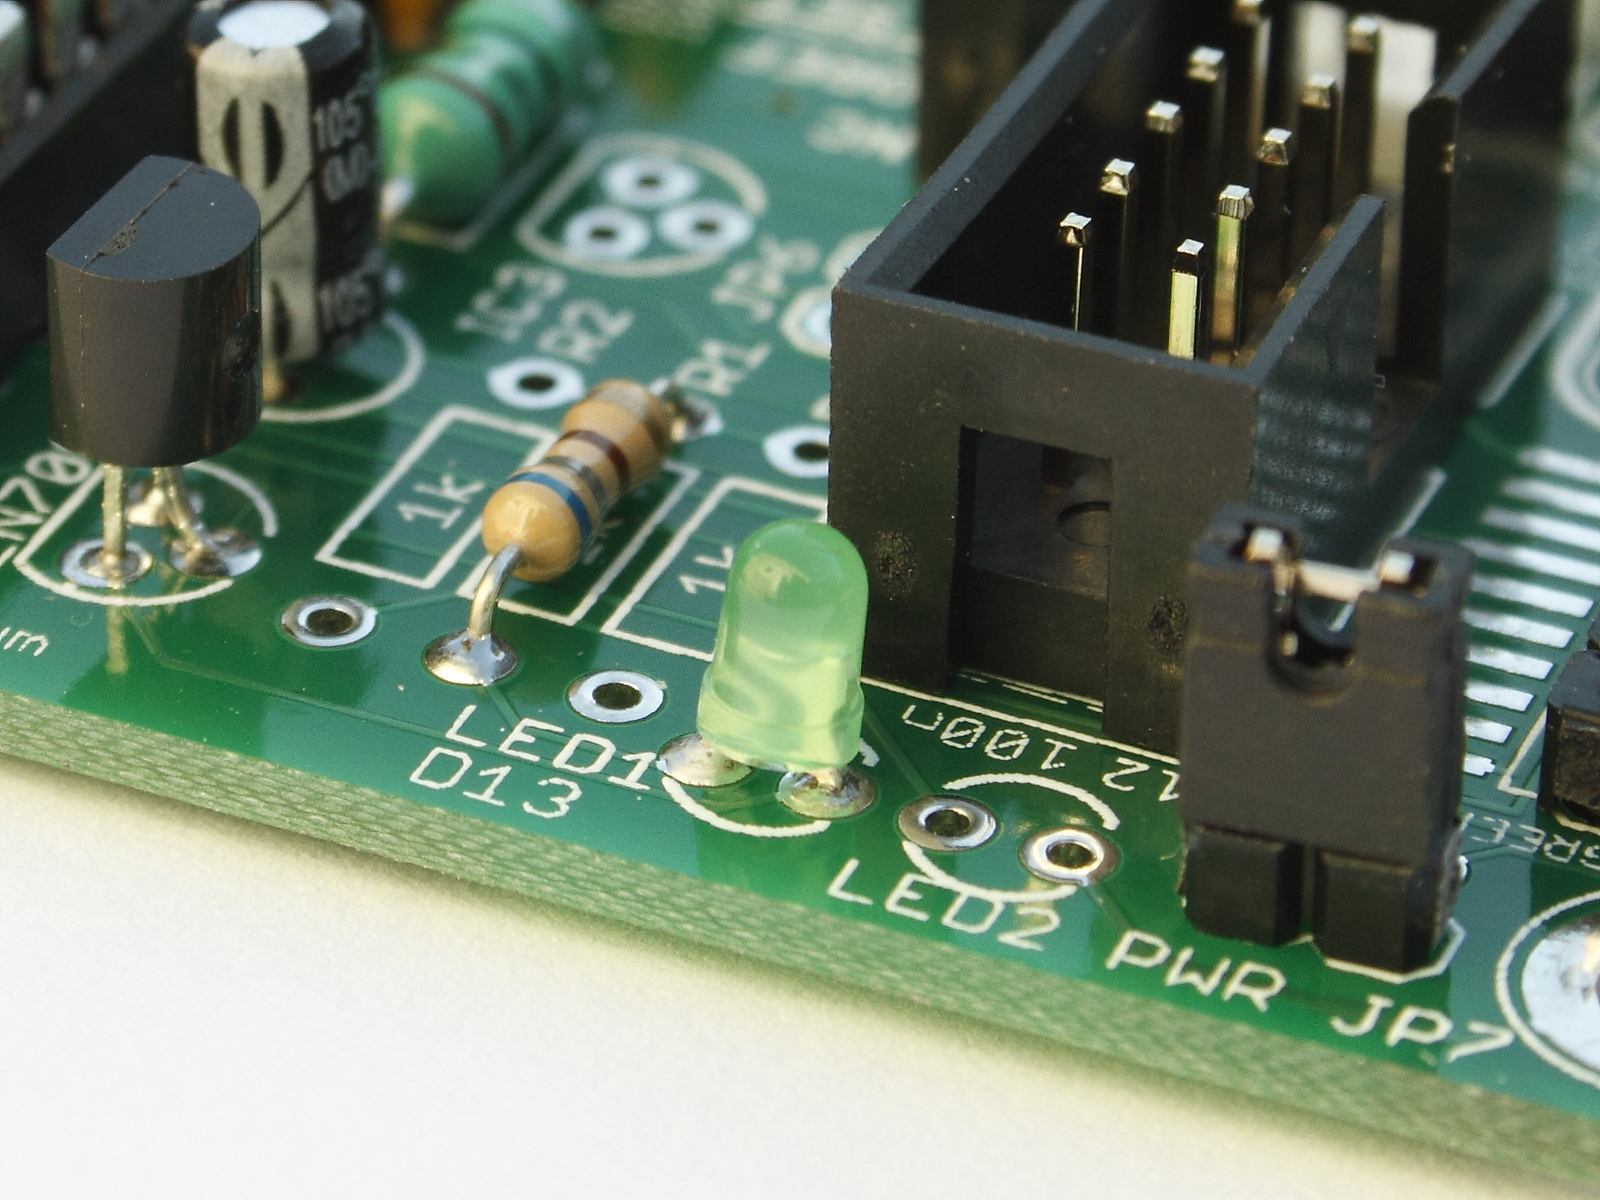
\includegraphics[keepaspectratio,width=10cm]{%
    images/calunium-led-orientation}
  \caption[LED orientation]{\led\ orientation. \photoCredit{%
      Steve Marple}{\ccBySaTwo}{%
      http://www.flickr.com/photos/stevemarple/10786846715/}}
  \label{fig:led-orientation}
\end{figure}
\begin{figure}
  \centering
  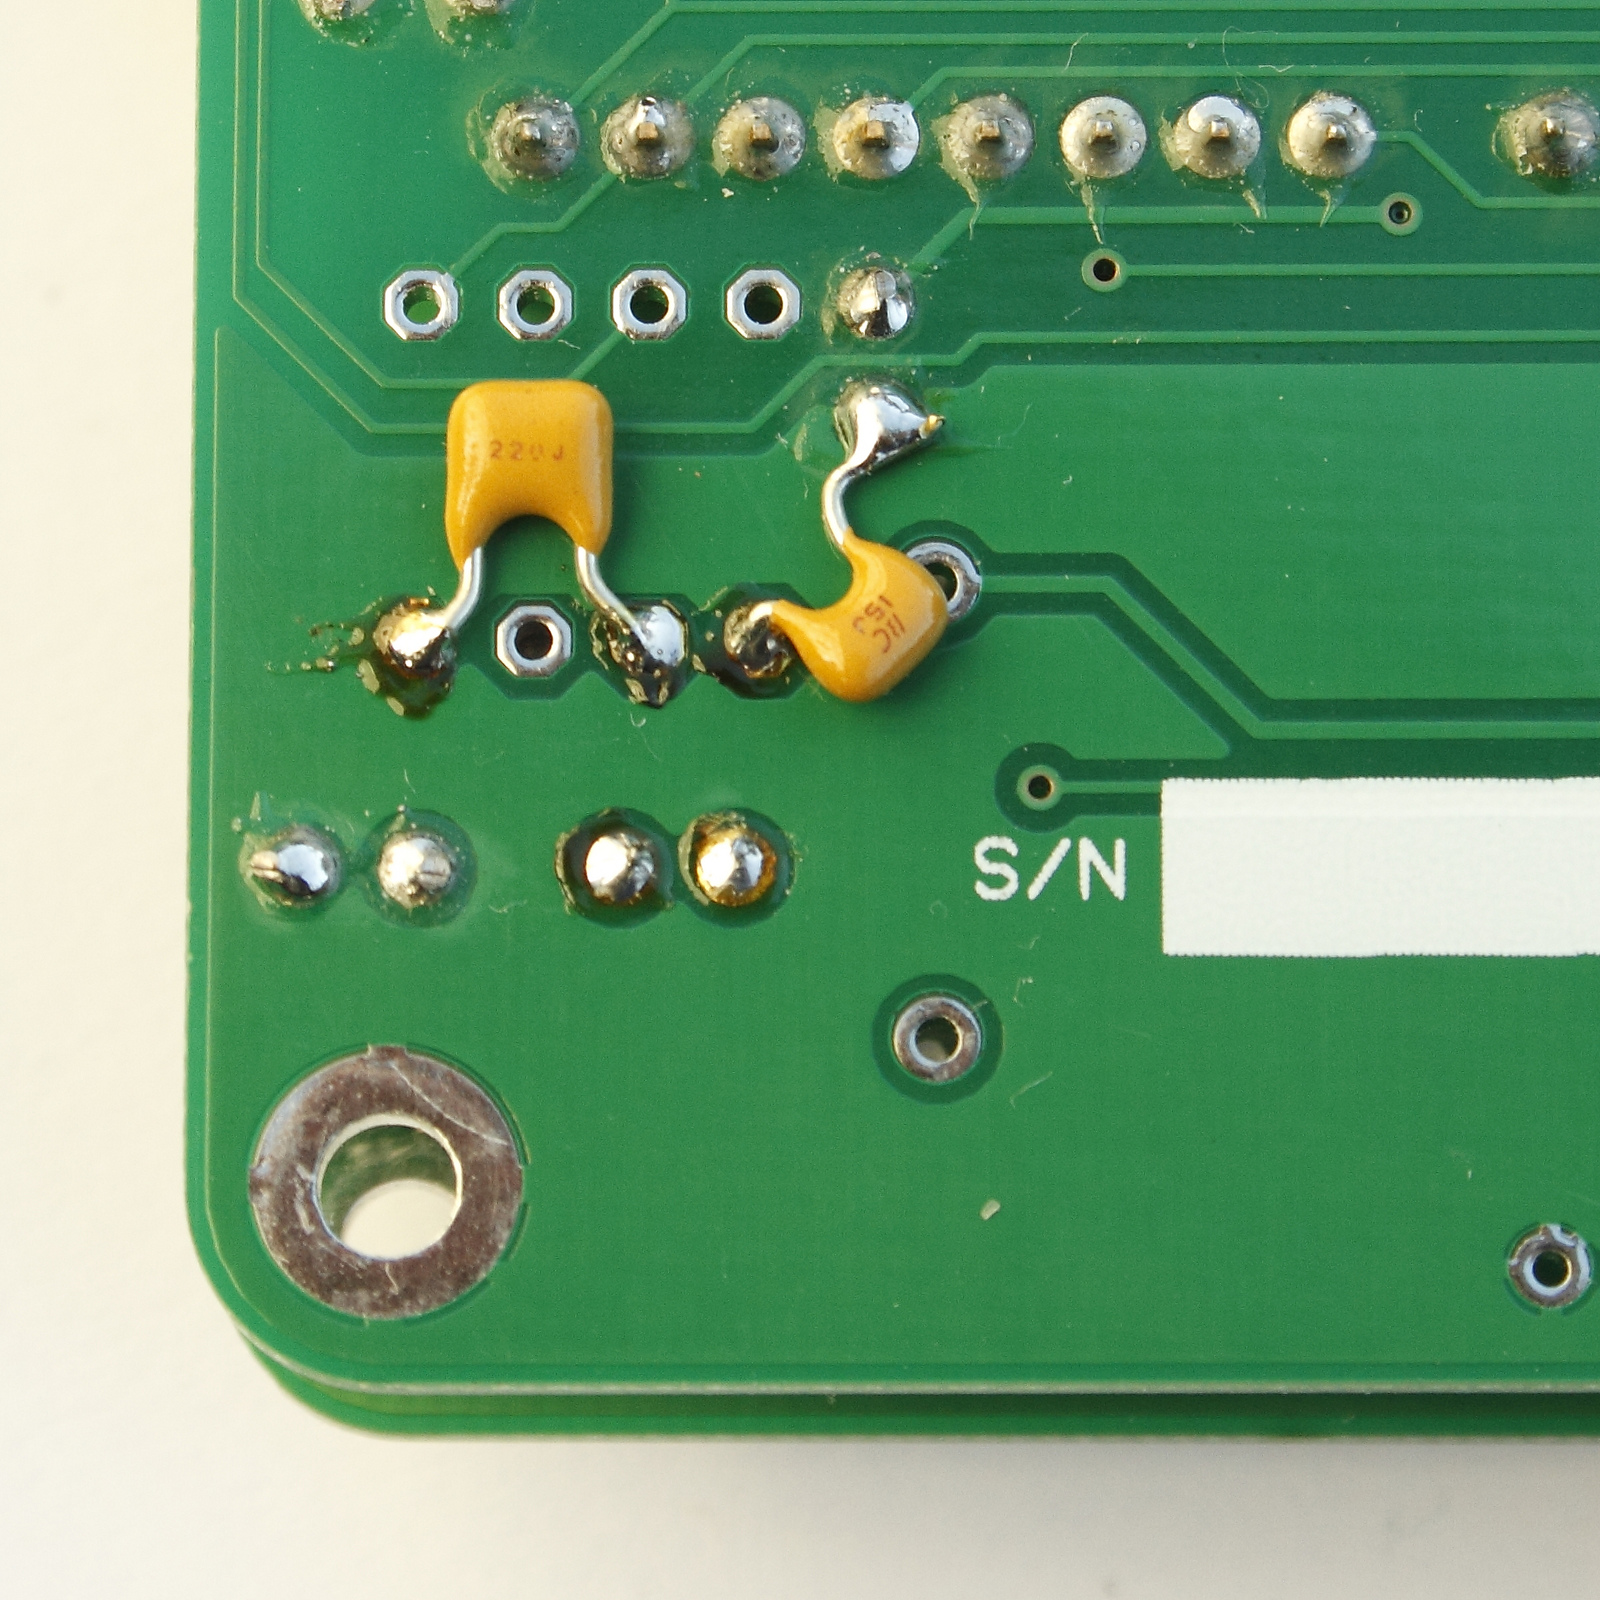
\includegraphics[keepaspectratio,width=10cm]{%
    images/calunium-rtc-caps-hack}
  \caption[Real-time clock load capacitors (Calunium v~2.0)]{%
    Real-time clock load capacitors (Calunium v~2.0). \photoCredit{%
      Steve Marple}{\ccBySaTwo}{%
      http://www.flickr.com/photos/stevemarple/10787041263/}}
  \label{fig:calunium-rtc-caps-hack}
\end{figure}


\begin{landscape}
  \begin{figure}[p]
    \centering
    \includegraphics[keepaspectratio,width=28cm,height=16cm]{%
      ../../hardware/Calunium/hardware/pcb/Calunium_v2/Calunium_v2_sch}  
    \caption{Calunium v.~2.0 circuit diagram.}
    \label{fig:calunium-v2.0-cct-diag}
  \end{figure}
  \begin{figure}[p]
    \centering
    % Use symbolic link for image to avoid a filename with a dot in
    % the main part of the name. This enables the extension to be left
    % off for easy processing with either latex or pdflatex.
    \includegraphics[keepaspectratio,width=28cm,height=16cm]{%
      images/Calunium_v2_1_sch}
    \caption{Calunium v.~2.1 circuit diagram.}
    \label{fig:calunium-v2.1-cct-diag}
  \end{figure}
\end{landscape}

\section{Testing the board}

\section{Programming the firmware}

These instructions assume you are using the Atmel AVR Dragon in \isp\
mode but adapting them to suit your programmer should be
straightforward; see the \filename{avrdude} manual page for further
information.

\subsection{Programming the bootloader}

Power up the Calunium board and connect the programmer. Ensure the
cable is correctly orientated at both ends. The bootloader can be
compiled and programmed simply, as user \piUser: \todo[Check directory]
\begin{Cmd}
  cd /home/pi/xboot
  make clean
  make SHELL=bash calunium_8MHz_RC_ISP.conf.mk program
\end{Cmd}
\todo: ignore lock bit verification errors.

If the bootloader is correctly programmed the green \led\ connected to
D13 on the Calunium \pcb\ should flash at about \Hz{1}.

\subsection{Programming the magnetometer firmware}
Ensure that the shunt marked ``AUTO RST'' is fitted, and that the
shunt marked ``FTDI PWR'' is omitted. Connect the FTDI cable and
identify the USB device file; as user \piUser:
\begin{Cmd}
  dmesg | tail
\end{Cmd}

Look for a line containing text similar to
\begin{Cmd}
  FTDI USB Serial Device converter now attached to ttyUSB0
\end{Cmd}
For the case above the device file \filename{/dev/ttyUSB0}. Now
program the microcontroller using the xboot bootloader. Replace
\filename{/dev/ttyUSB0} with the device file one your system. As user
\piUser:
\begin{Cmd}
  cd /home/pi/AuroraWatchNet/firmware/magnetometer
  avrdude -p atmega1284p -b 38400 -c avr109 -P /dev/ttyUSB0 \textbackslash
      -U flash:w:xrf_rf12-0.10a.bin:r
\end{Cmd}


\helpbox{Whilst it is possible to program the firmware using the AVR
  Dragon alone this approach ensures that the xboot bootloader is
  present and functions correctly, allowing the microcontroller
  firmware to be updated over the radio link.}

\chapter{Sensor PCB assembly}

\section{Sensor PCB version 1.2}

\subsection{Order of assembly}
Fit components in order:
\begin{buildorder}
\item Turned pin sockets for the FLC100 sensor. Accurate alignment is
  important so use a peice of solderless breadboard to hold the male
  turned-pin headers (\figurename~\ref{fig:flc100-step-1}). Insert the
  headers so that the conical part is pointing downwards. Fit the
  upside down turned-pin sockets onto the headers
  (\figurename~\ref{fig:flc100-step-2}). Place the PCB onto the
  upside-down sockets (\figurename~\ref{fig:flc100-step-3}) and solder
  all 7 connections. Remove from the breadboard, leaving the male
  headers in place. Carefully position the FLC100 sensor onto the male
  turned-pin headers. The top-side of the FLC100 has two yellow
  capacitors and the letters BS the circuit board. Solder the FLC100
  sensor to the header. Gently remove the FLC100 sensor and place in
  an anti-static bag.
  \begin{figure}[p]
    \centering
    \todo[Take photo and insert]
    %%\includegraphics[width=10cm,keepaspectratio]{%
     %% images/flc100-step-1}
    \caption{Fit the male turned-pin headers.}
    \label{fig:flc100-step-1}
  \end{figure}
  \begin{figure}[p]
    \centering
    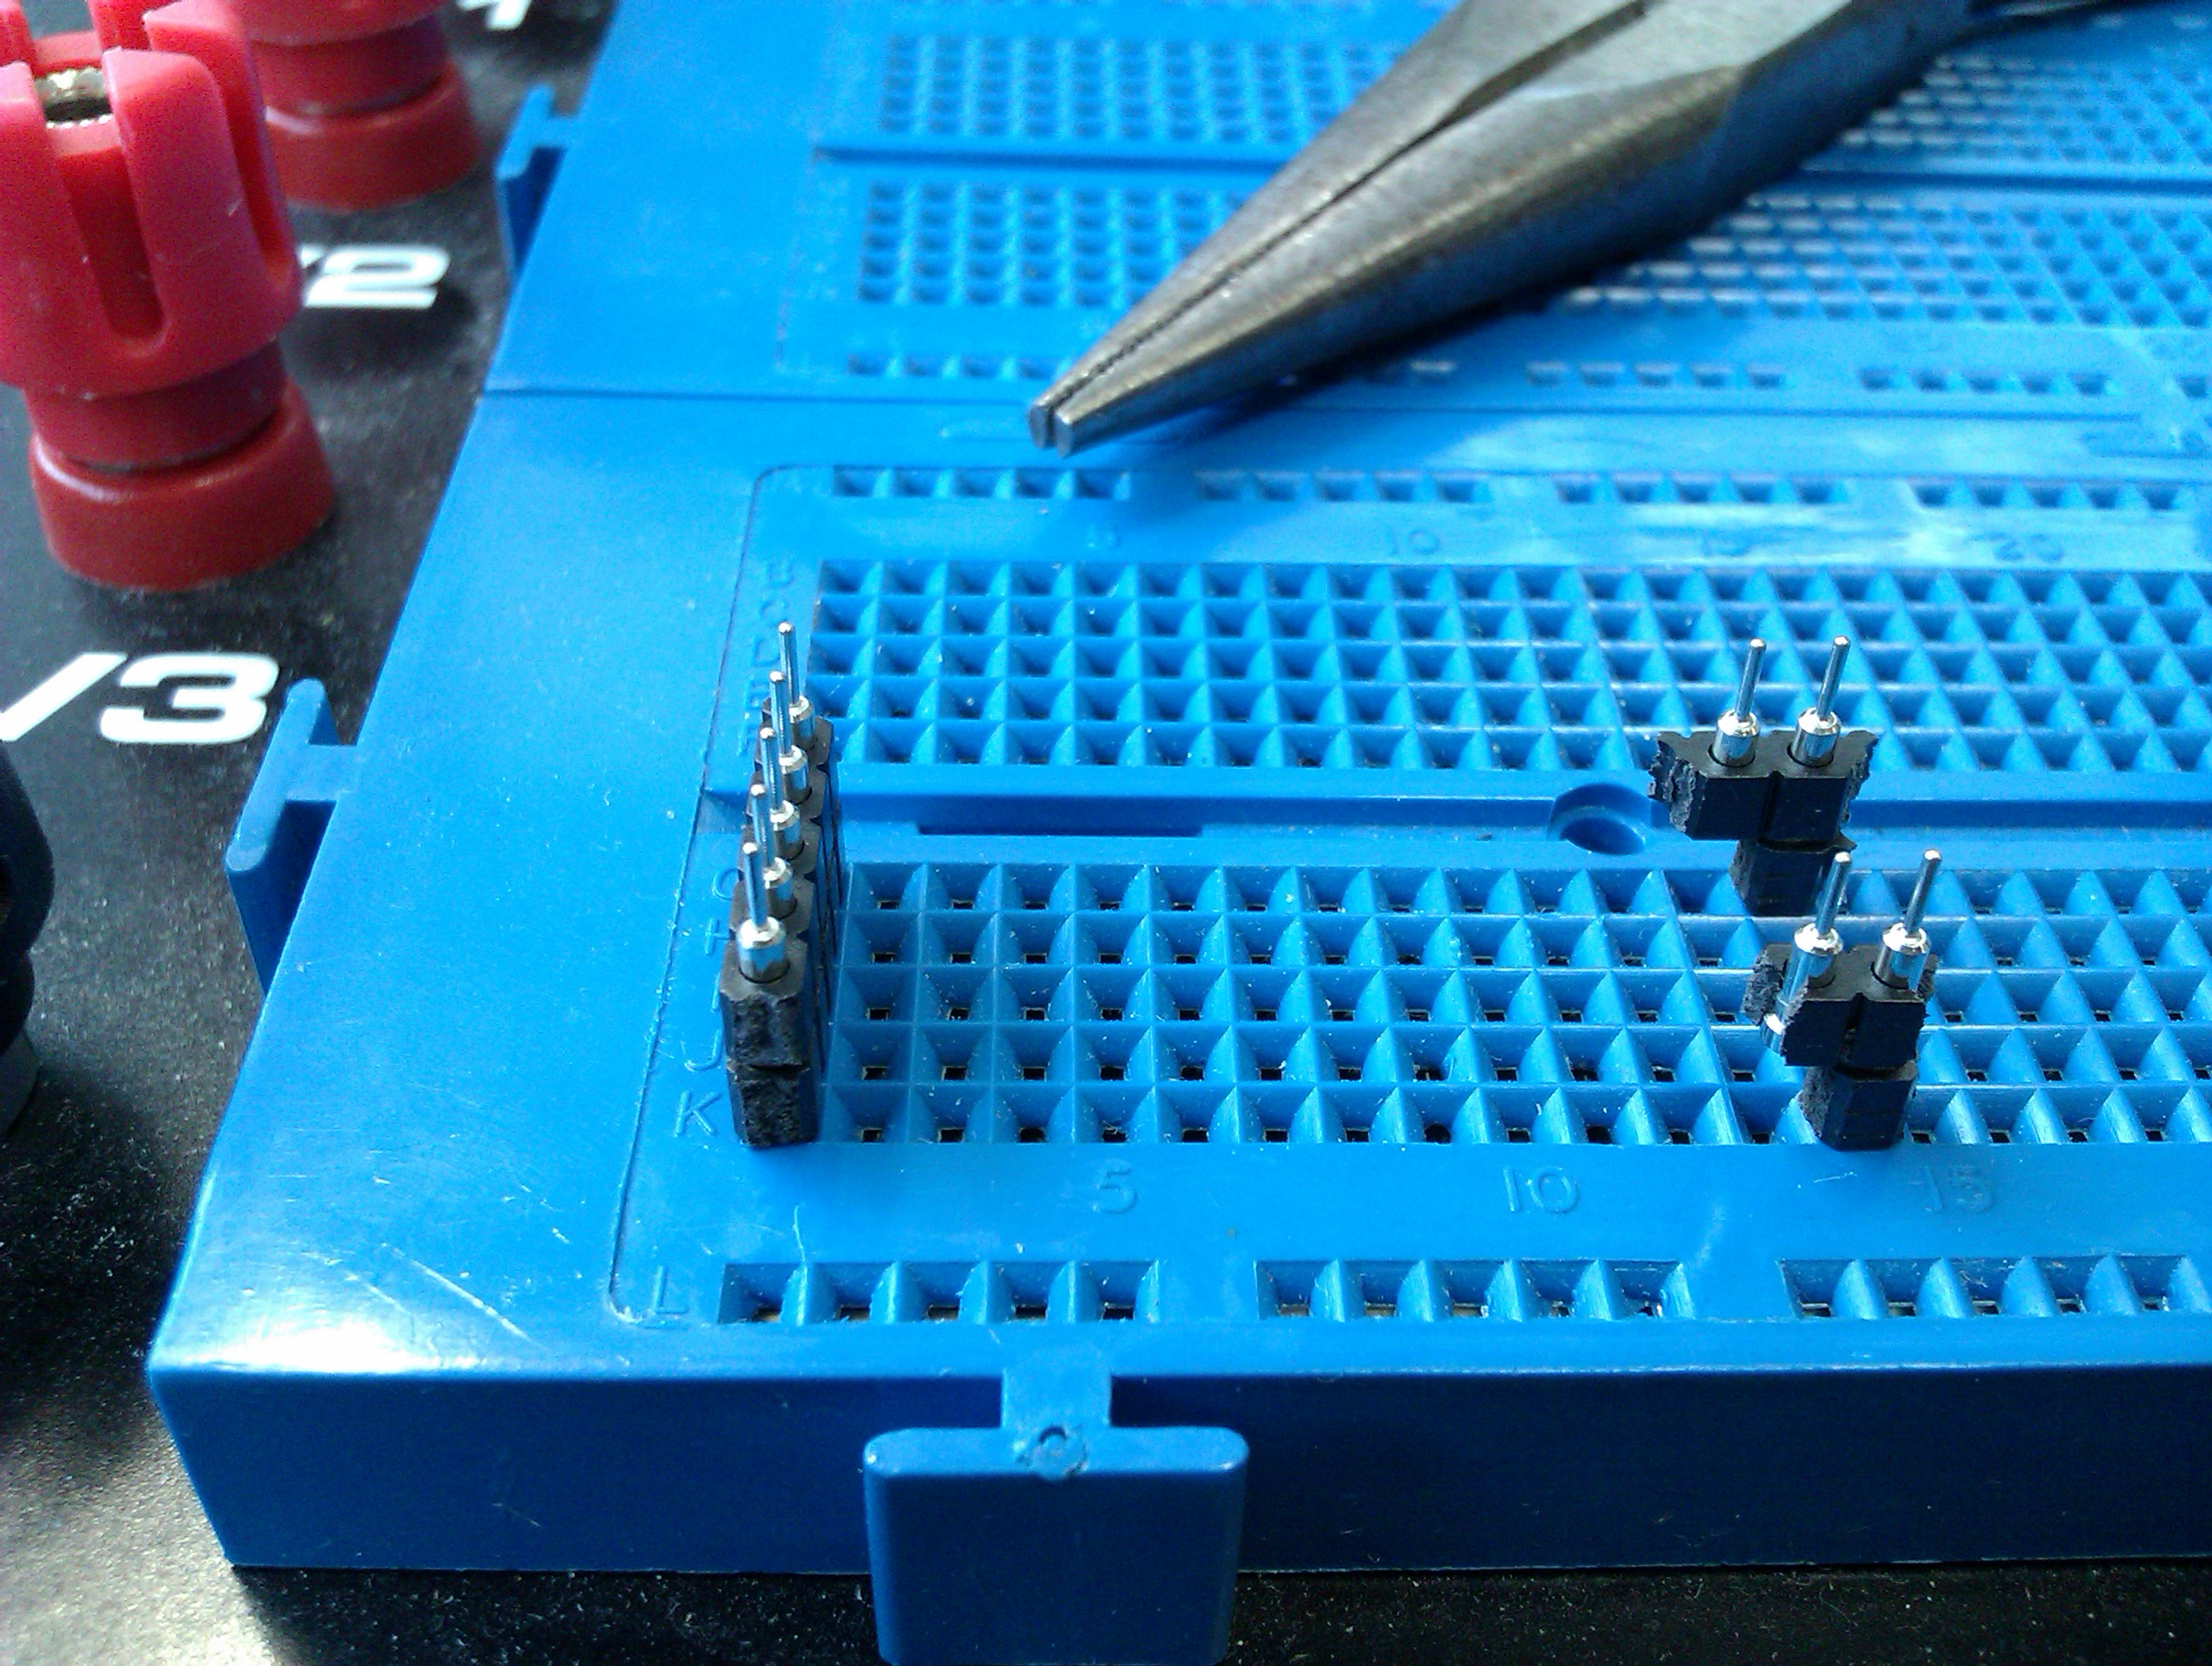
\includegraphics[width=10cm,keepaspectratio]{%
      images/flc100-step-2}
    \caption{Fit the female turned-pin sockets.}
    \label{fig:flc100-step-2}
  \end{figure}
  \begin{figure}[p]
    \centering
    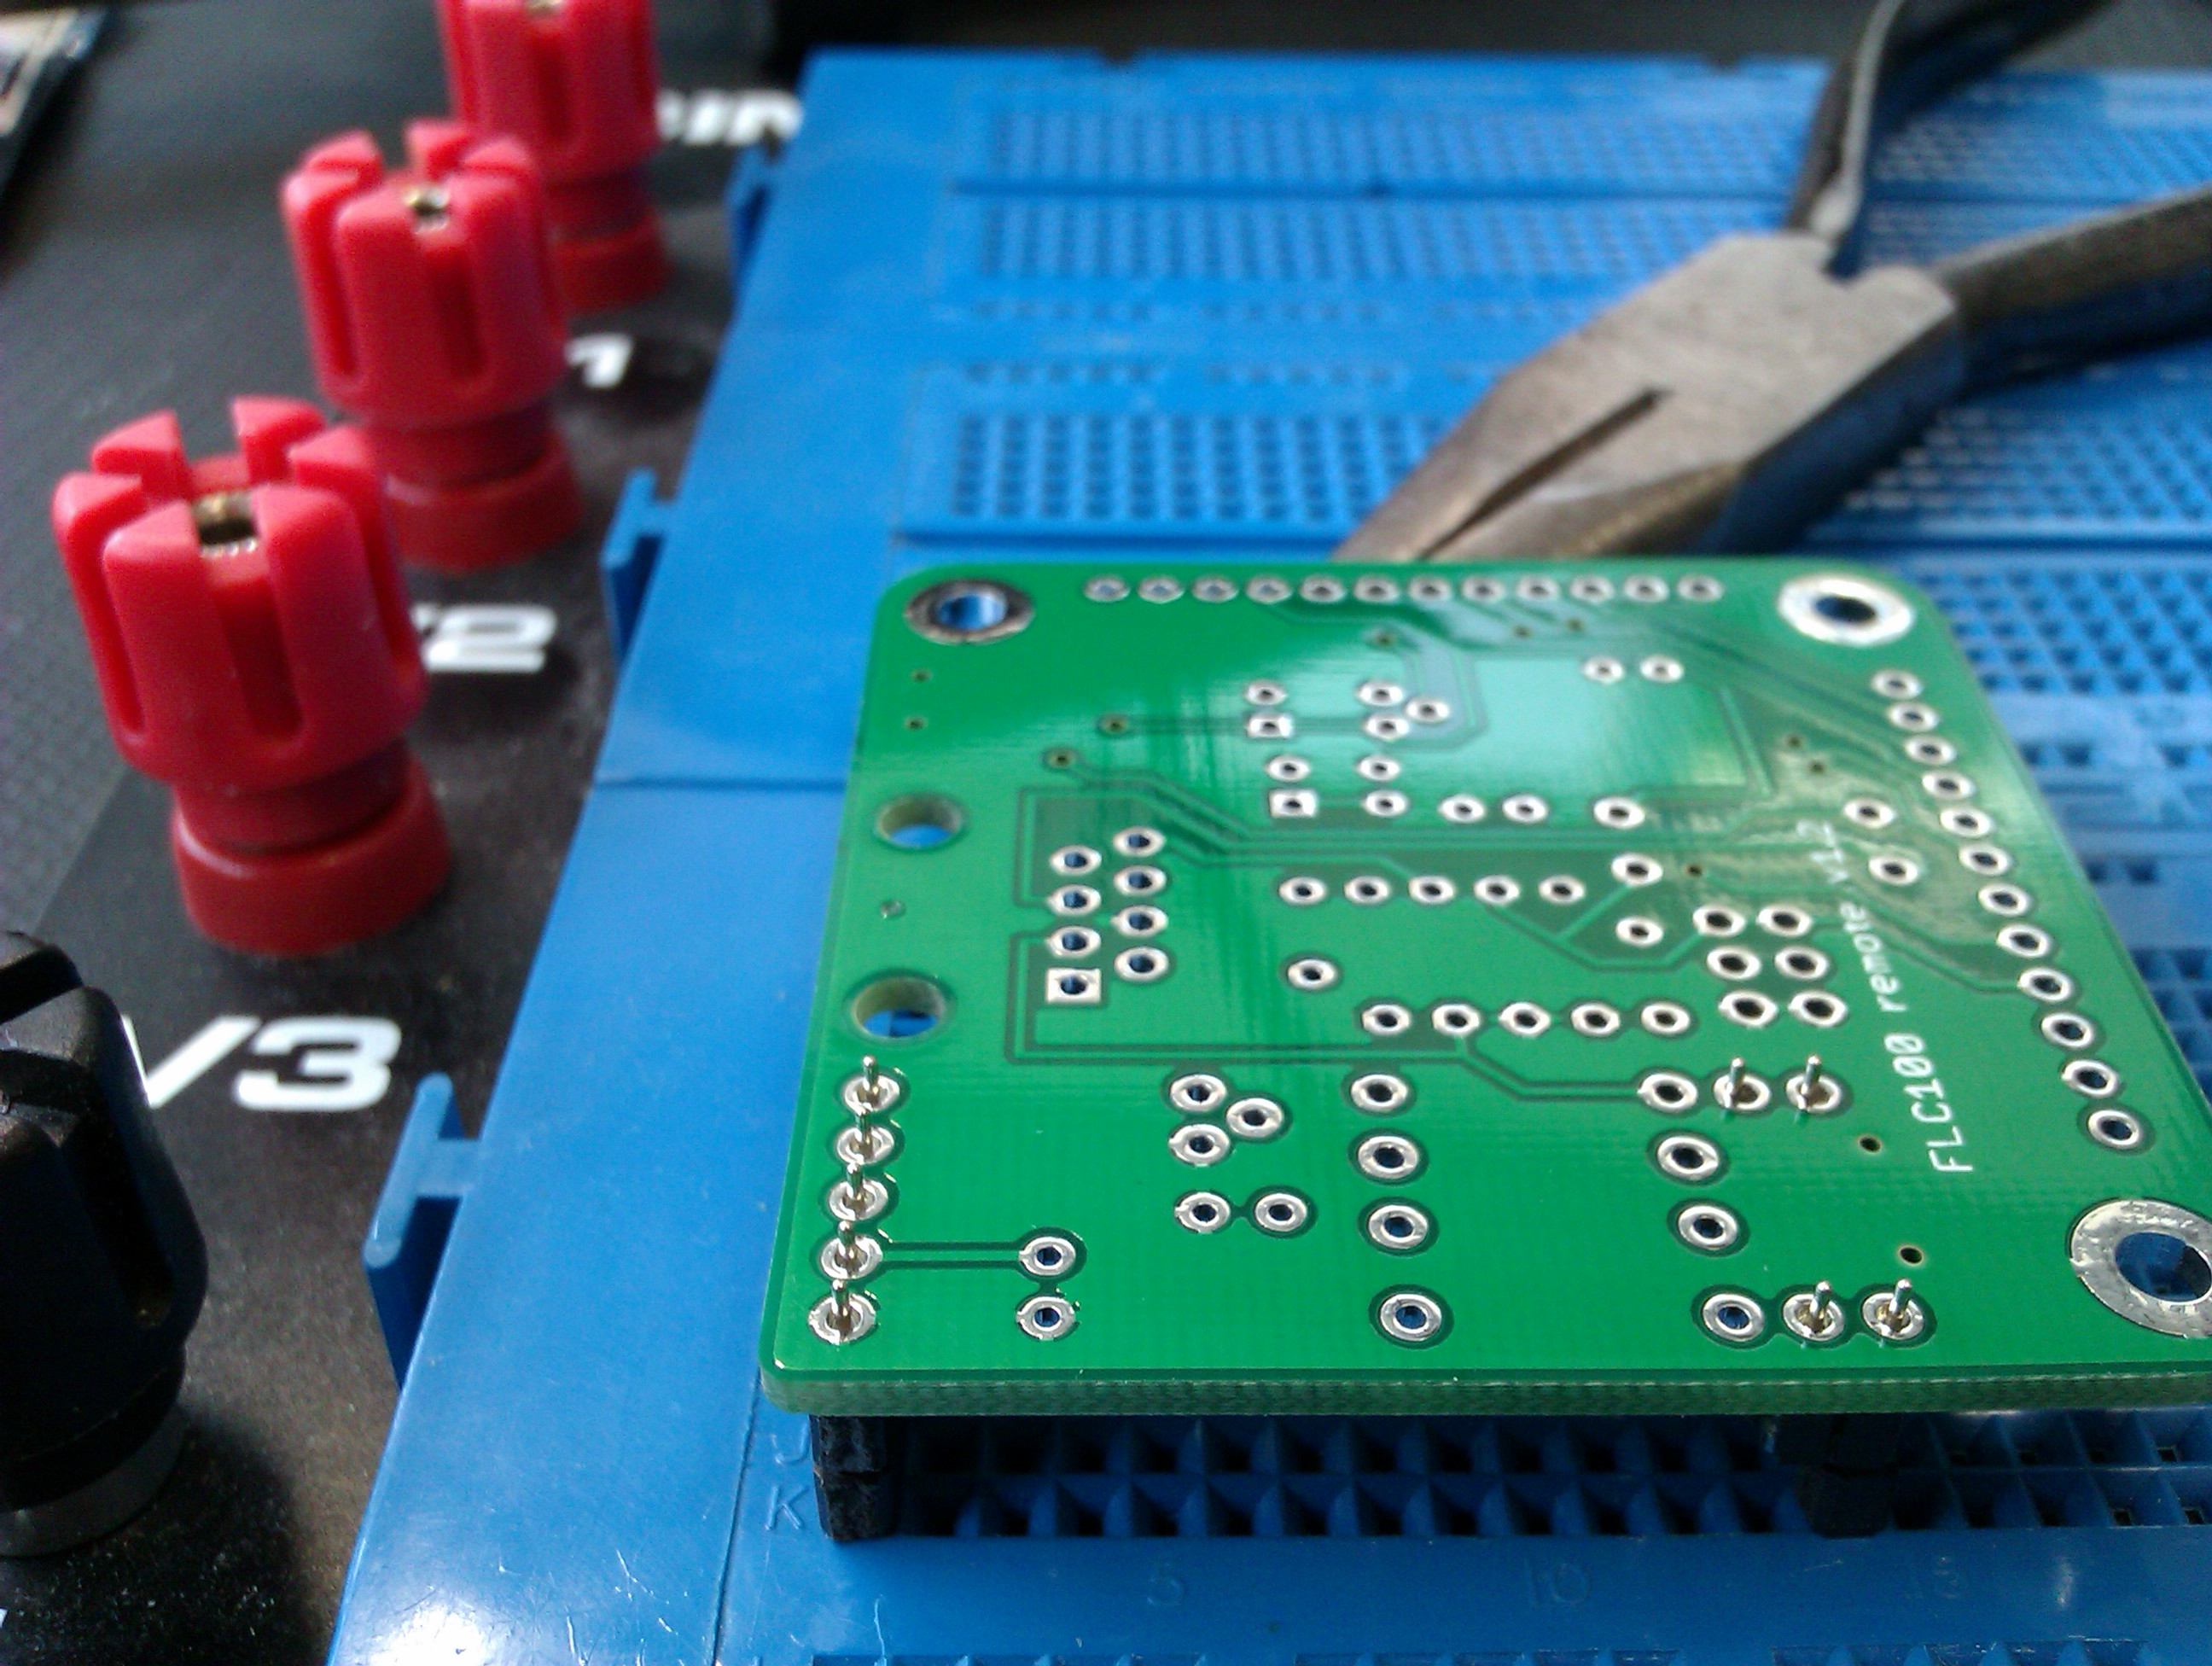
\includegraphics[width=10cm,keepaspectratio]{%
      images/flc100-step-3}
    \caption[Place the sensor PCB onto the female turned-pin
    sockets.]{%
      Place the sensor PCB onto the female turned-pin sockets. The
      pliers are used to support the other side of the PCB.}
    \label{fig:flc100-step-3}
  \end{figure}
\item IC1 (MAXMCP3424).
\item IC2 (MAX619).
\item R1, R2, R3 (\kohm{10}).
\item R4 (\kohm{100}).
\item R5 (\kohm{4.7}).
\item C1, C2, C5, C9 (\nF{100}).
\item C9 (\nF{10}).  
\item C6, C7 (\nF{220}).
\item C3, C4 (\uF{4.7}).
\item D1 (BAT85).
\item SENS2 (LM61).
\item JP5 and JP7 (fit as $2\times3$ male header).
\item X1 (RJ45 vertical jack).
\item Q1 (2N7000). This item is very sensitive to damage by
  electrostatic discharge!
\item SENS1. Gently fit the FLC100 sensor into the turned-pin
  sockets. Apply pressure only on the circuit boards, not the
  components or coil.
\end{buildorder}

\begin{landscape}
  % \thispagestyle{empty}
  \begin{figure}[p]
    \centering
    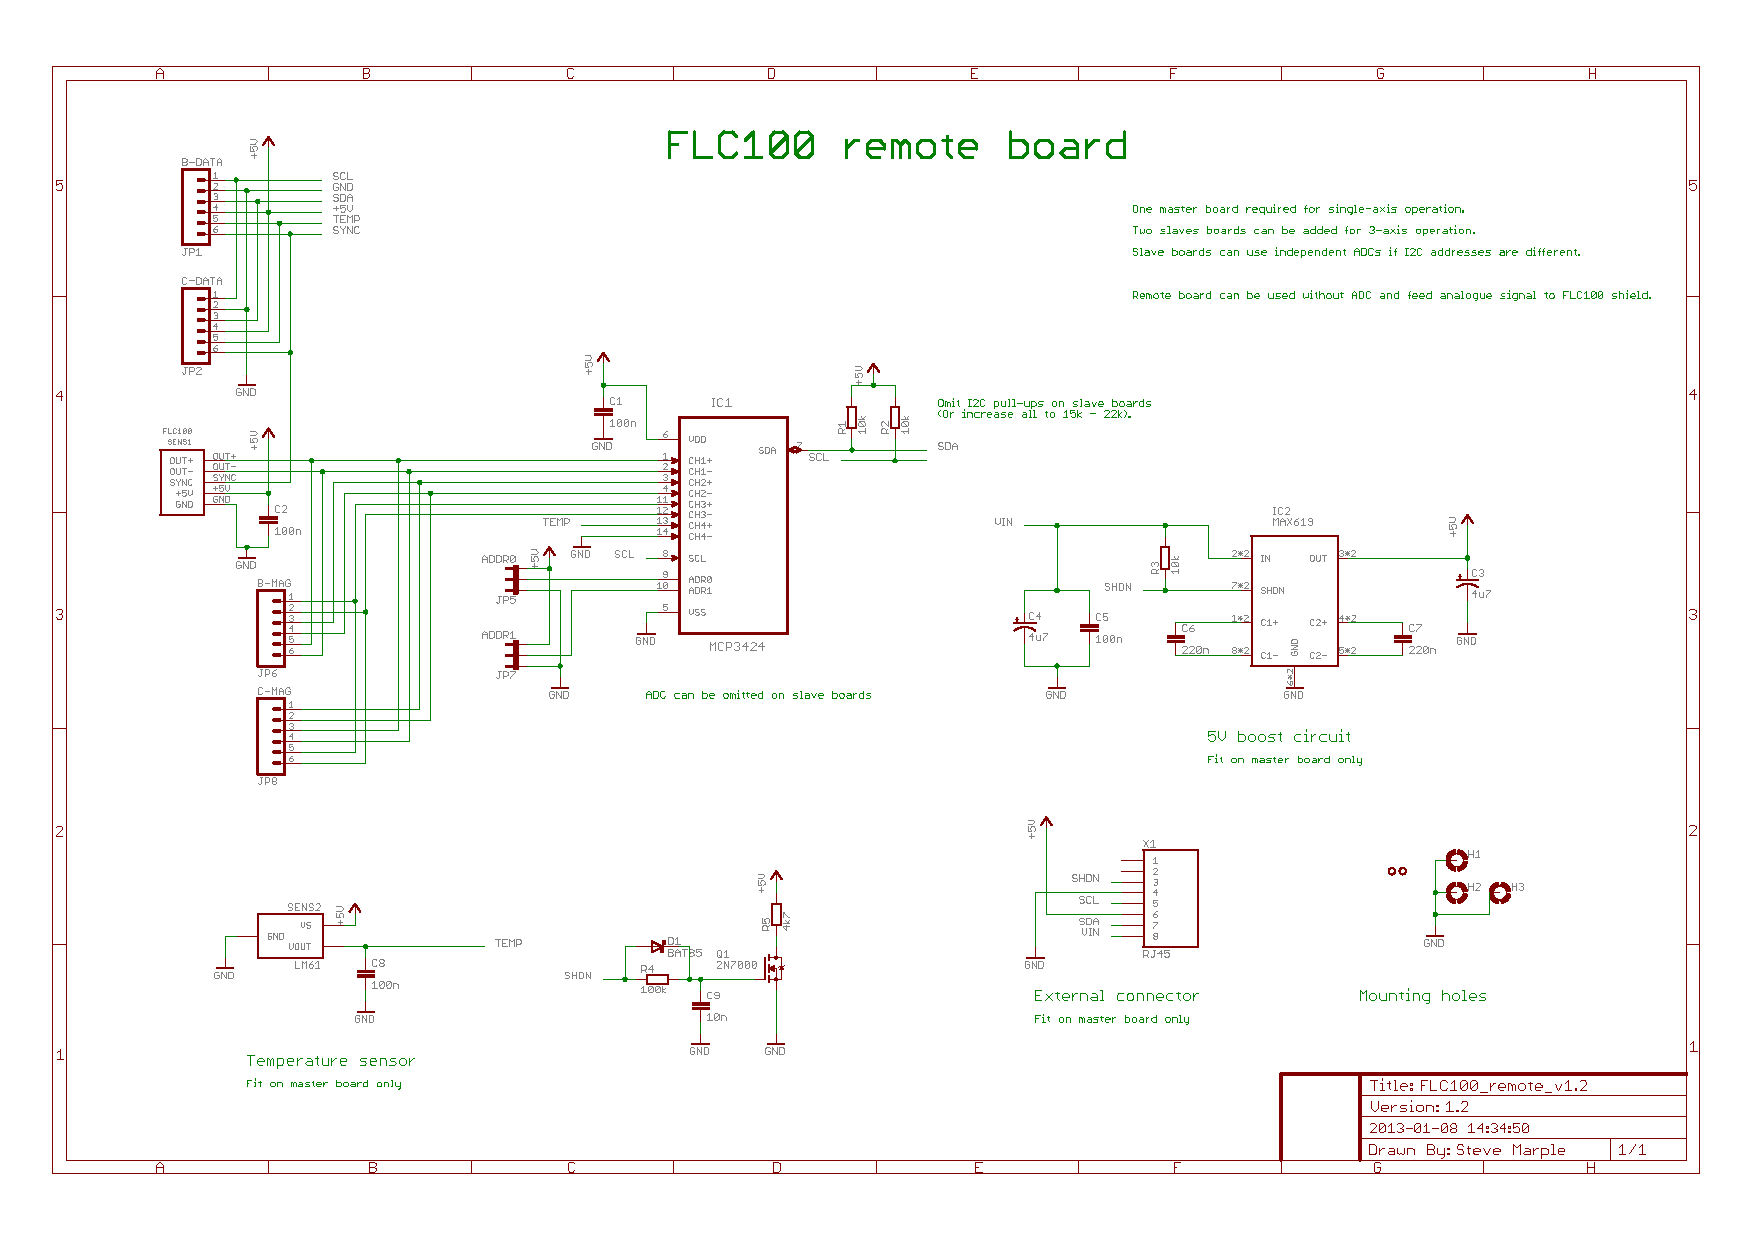
\includegraphics[keepaspectratio,width=28cm,height=16cm]{%
      {../../hardware/FLC100_shield/remote_v1.2/FLC100_remote_v1.2_sch}.pdf}
    \caption{Sensor PCB version 1.2 circuit diagram.}
    \label{fig:sensor-v1.2-pcb-cct-diag}
  \end{figure}
\end{landscape}


\part{Installation}

\chapter{Site requirements}

\section{Sensor requirements}
The site for the sensor should be chosen with regard to the following
requirements (highest priority given first).

\begin{itemize}
\item Within range of the base unit.
\item Away from moving metal objects, for example, trains (more than
  \SI{50}{\metre}), cars (more than \SI{20}{\metre}).
\item Away from static metal objects, in particular those containing
  the \emph{ferro-magnetic} materials iron, nickel and cobalt.
\end{itemize}

\section{Network requirements}

The following network requirements are needed for the system to
operate fully:
\begin{itemize}
\item \dns\ resolution. This is normally provided
  as standard on most networks.
\item Outgoing access on port 123 (\ntp).
\item Outgoing \ssh\ access (port 22).
\end{itemize}





\chapter{Raspberry Pi setup}

\section[SD card creation]{\sd\ card creation}

Download the latest Raspbian image and copy to the \sd\ card following
the instructions on the Raspberry Pi web site. \textbf{Copying
  the compressed image to a FAT partition on the \sd\ card will not work}.

\section{Configuring Raspbian}

\helpbox{In the command window you can press the \keypress{Tab} key
  to have Linux complete the command or filename.}

Raspbian is most easily configured by booting the new image. If you
are able to discover the \ip\ address (for instance, by checking the
\dhcp\ tables of your home router) you can do this over the network
using \ssh. Otherwise you must use attach a keyboard and monitor to the
Raspberry Pi. If you are familiar with Linux it is also possible to
edit the files by mounting the \sd\ card on another Linux system.

\subsection{/dev/ttyAMA0 serial port setup}

Disable the console from running on \filename{/dev/ttyAMA0}. Edit
\filename{/boot/cmdline.txt} to remove the parts which relate to
\filename{ttyAMA0}. Remove
\begin{Cmd}
console=ttyAMA0,115200 kgdboc=ttyAMA0,115200
\end{Cmd}


Disable the \code{getty} process from running on
\filename{/dev/ttyAMA0}. Edit \filename{/etc/inittab}. Find the line
relating to \filename{ttyAMA0}. Either delete the line entirely or
comment it out by inserting a hash character (\#) at the start of the
line.

\subsection{Raspbian configuration}

Log in as \piUser\ and run
\begin{Cmd}
sudo raspi-config
\end{Cmd}

\subsubsection{Change user password}
\textbf{If the default password has not been changed then do so now to keep
your system secure.}

\subsubsection{Internationalisation options}
\filename{cron} uses local time and the shift to and from daylight
saving time complicates the \filename{cron} tables. Set the Raspberry
Pi's timezone to \utc\ to avoid daylight saving.

Select \code{Internationalisation Options} and
then \code{Change Timezone}. For geographic area select %
\code{None of the above}, then select \code{\utc}. Select \code{OK}.

\subsubsection{Advanced options}
Select \code{Advanced Options} and then \code{Memory
  Split}. Set the \gpu\ memory to \code{16} (MB).

\subsubsection{Expand Filesystem}
Finally select \code{Expand Filesystem}. Although the first option
do this last. Choose \code{Finish} and then reboot.

\section{Install missing software packages}
As user \rootUser
\begin{Cmd}
apt-get install screen lsof python-pip ipython python-matplotlib

dpkg -i ~pi/python-numpy_1.7.1-3_armhf.deb
\end{Cmd}

\section{Installing the AuroraWatchNet server software}

\subsection{Install the Git repository}
As user \piUser
\begin{Cmd}
git clone --recursive https://github.com/stevemarple/AuroraWatchNet.git 
git clone --recursive https://github.com/stevemarple/auroraplot.git
git clone --recursive https://github.com/stevemarple/Calunium.git
mkdir \mytilde/bin
cd \mytilde/bin
ln -s ../AuroraWatchNet/software/server/awnetd/awnetd.py
ln -s ../AuroraWatchNet/software/server/bin/log_ip
\end{Cmd}

\subsection{Configure \protect\filename{cron}}
\label{sec:cron-configuration}
As user \piUser
\begin{Cmd}
crontab -e
\end{Cmd}

In the \filename{nano} editor add the following lines: \todo[Add lines
for data transfer]
\begin{Cmd}
@reboot /home/pi/bin/log_ip reboot > /dev/null 2>&1
@hourly /home/pi/bin/log_ip > /dev/null 2>&1
\end{Cmd}
Save the file, \keystroke{CTRL}-\keystroke{x}, \keystroke{y},
\myreturn.

\subsection{Configure \protect\filename{ifplugd}}

As user \rootUser
\begin{Cmd}
cd /etc/ifplugd/action.d
ln -s /home/pi/AuroraWatchNet/software/server/bin/log_ip
\end{Cmd}

\subsection{Create configuration file}

As user \rootUser
\begin{Cmd}
mkdir /data
chown pi.pi /data
nano /etc/awnet.ini
\end{Cmd}

\todo[Create file contents, perhaps using a template copied from
the repository]

\subsection{Create init file for server daemon}
As user \rootUser
\begin{Cmd}
cd /etc/init.d
ln -s /home/pi/AuroraWatchNet/software/server/awnetd/awnetd.sh awnetd
update-rc.d  awnetd defaults
\end{Cmd}

\subsection{Configure \protect\filename{ntp}}
\todo[May not be necessary for most users, but all users should check
that the time is correct]


\part{Operation}
\chapter{Raspberry Pi operation}

\section{Introduction}

For generic operation of the Raspberry Pi (setting the hostname,
assigning a fixed \ip\ address \etc) please see the Raspbian
documentation,
\url{http://www.raspbian.org/RaspbianDocumentation}.

\section{Shutting down the Raspberry Pi}

The Raspberry Pi must be shutdown cleanly before power is removed:
\begin{Cmd}
sudo shutdown -h now
\end{Cmd}
Before removing the power wait until only the red power \led\ is lit;
wait a further two seconds to ensure futher access to the \sd\ card is
not needed. If the power is removed whilst data is being written to
the \sd\ card it will corrupt the file system.


To reboot the Raspberry Pi use
\begin{Cmd}
sudo shutdown -r now
\end{Cmd}

\section{Starting and stopping the data recording daemon}

Data is recorded on the Raspberry Pi using a \emph{daemon} process,
which is started and stopped by the Debian init scripts. The scripts
must be started and stopped as user \rootUser, the actual data
recording process runs as user \piUser.

To start data recording
\begin{Cmd}
sudo /etc/init.d/awnetd start
\end{Cmd}

To stop data recording
\begin{Cmd}
sudo /etc/init.d/awnetd stop
\end{Cmd}

It is also possible to check the status of the data recording process
\begin{Cmd}
sudo /etc/init.d/awnetd status
\end{Cmd}

\label{awnetd-restart}
The \code{restart} option forcibly stops recording (if running) and
then starts it again:
\begin{Cmd}
sudo /etc/init.d/awnetd restart
\end{Cmd}

\section{Monitoring the data recording process}
\label{monitor-daemon-output}
The data recording process directs its standard output and error
streams to a virtual terminal using \code{screen}. It is possible to
attach to this virtual terminal to monitor the output.

As user \piUser
\begin{Cmd}
screen -r awnet
\end{Cmd}

To exit from \code{screen} type \keystroke{CTRL}-\keystroke{a},
\keystroke{d}. 

\warningbox{Pressing \keystroke{CTRL}-\keystroke{c} will terminate the recording
  process.}





\chapter{Software and firmware updates}

\section{Raspbian updates}
\todo[See Raspberry Pi web pages]

\section{AuroraWatchNet software updates}
\label{awn-software-updates}

The software can be updated easily simply by \emph{pulling} a new
version from the Github repository. As user \piUser
\begin{Cmd}
cd \mytilde/AuroraWatchNet
git pull
\end{Cmd}

\section{Sensor unit firmware updates}
Only apply firmware updates if they are necessary. The firmware
version selected must match the hardware, if it does not the sensor
unit will be left inoperable and recovery will require an in-circuit
serial programmer. First ensure that the AuroraWatchNet software has
been updated (section~\ref{awn-software-updates}) and the recording
process restarted (section~\ref{awnetd-restart}). To update the
firmware
\begin{Cmd}
send_cmd.py --upgradeFirmware=\textsl{name-version}
\end{Cmd}
Replace \textsl{name-version} with the firmware name\slash version
string.


%%\appendix

%%\include{custom-ras-pi-imagaes}
\end{document}

